\documentclass[12pt]{article}

\usepackage{amsmath}
\usepackage{amssymb}

\usepackage{graphicx}

\begin{document}


Goals: 
\begin{itemize}
\item Want to examine the effects of the scale of the noise on NIV
\item Will look at systems with both underlying noise in the ``intrinsic'' variables, and added noise to the variables in the transformed/ ``ambient'' space
\item The magnitude of the noise in the ambient space will determine the embedding we compute
\item We expect to obtain DMAPS variables if the noise in the ambient space is large (we will only ``see'' the ambient space noise, and not the , and NIV if the noise in the ambient space is small
\end{itemize}


Assume we have the following underlying dynamical system (two--dimensional Brownian motion)
\begin{eqnarray}
	dx_1 & = & dW_1 \\
	dx_2 & = & dW_2
\end{eqnarray}
where $W_1, W_2$ are independent Browinain motions, $x_1, x_2 \in [0, 1]$, and we impose reflective boundary conditions.

We then apply following nonlinear transformation
%
\begin{eqnarray}
y_1 & = & x_1 + x_2^3 \\
y_2 & = & x_2 - x_1^3
\end{eqnarray}
%
The data are shown in Figure \ref{fig:data}

\begin{figure}[htb]
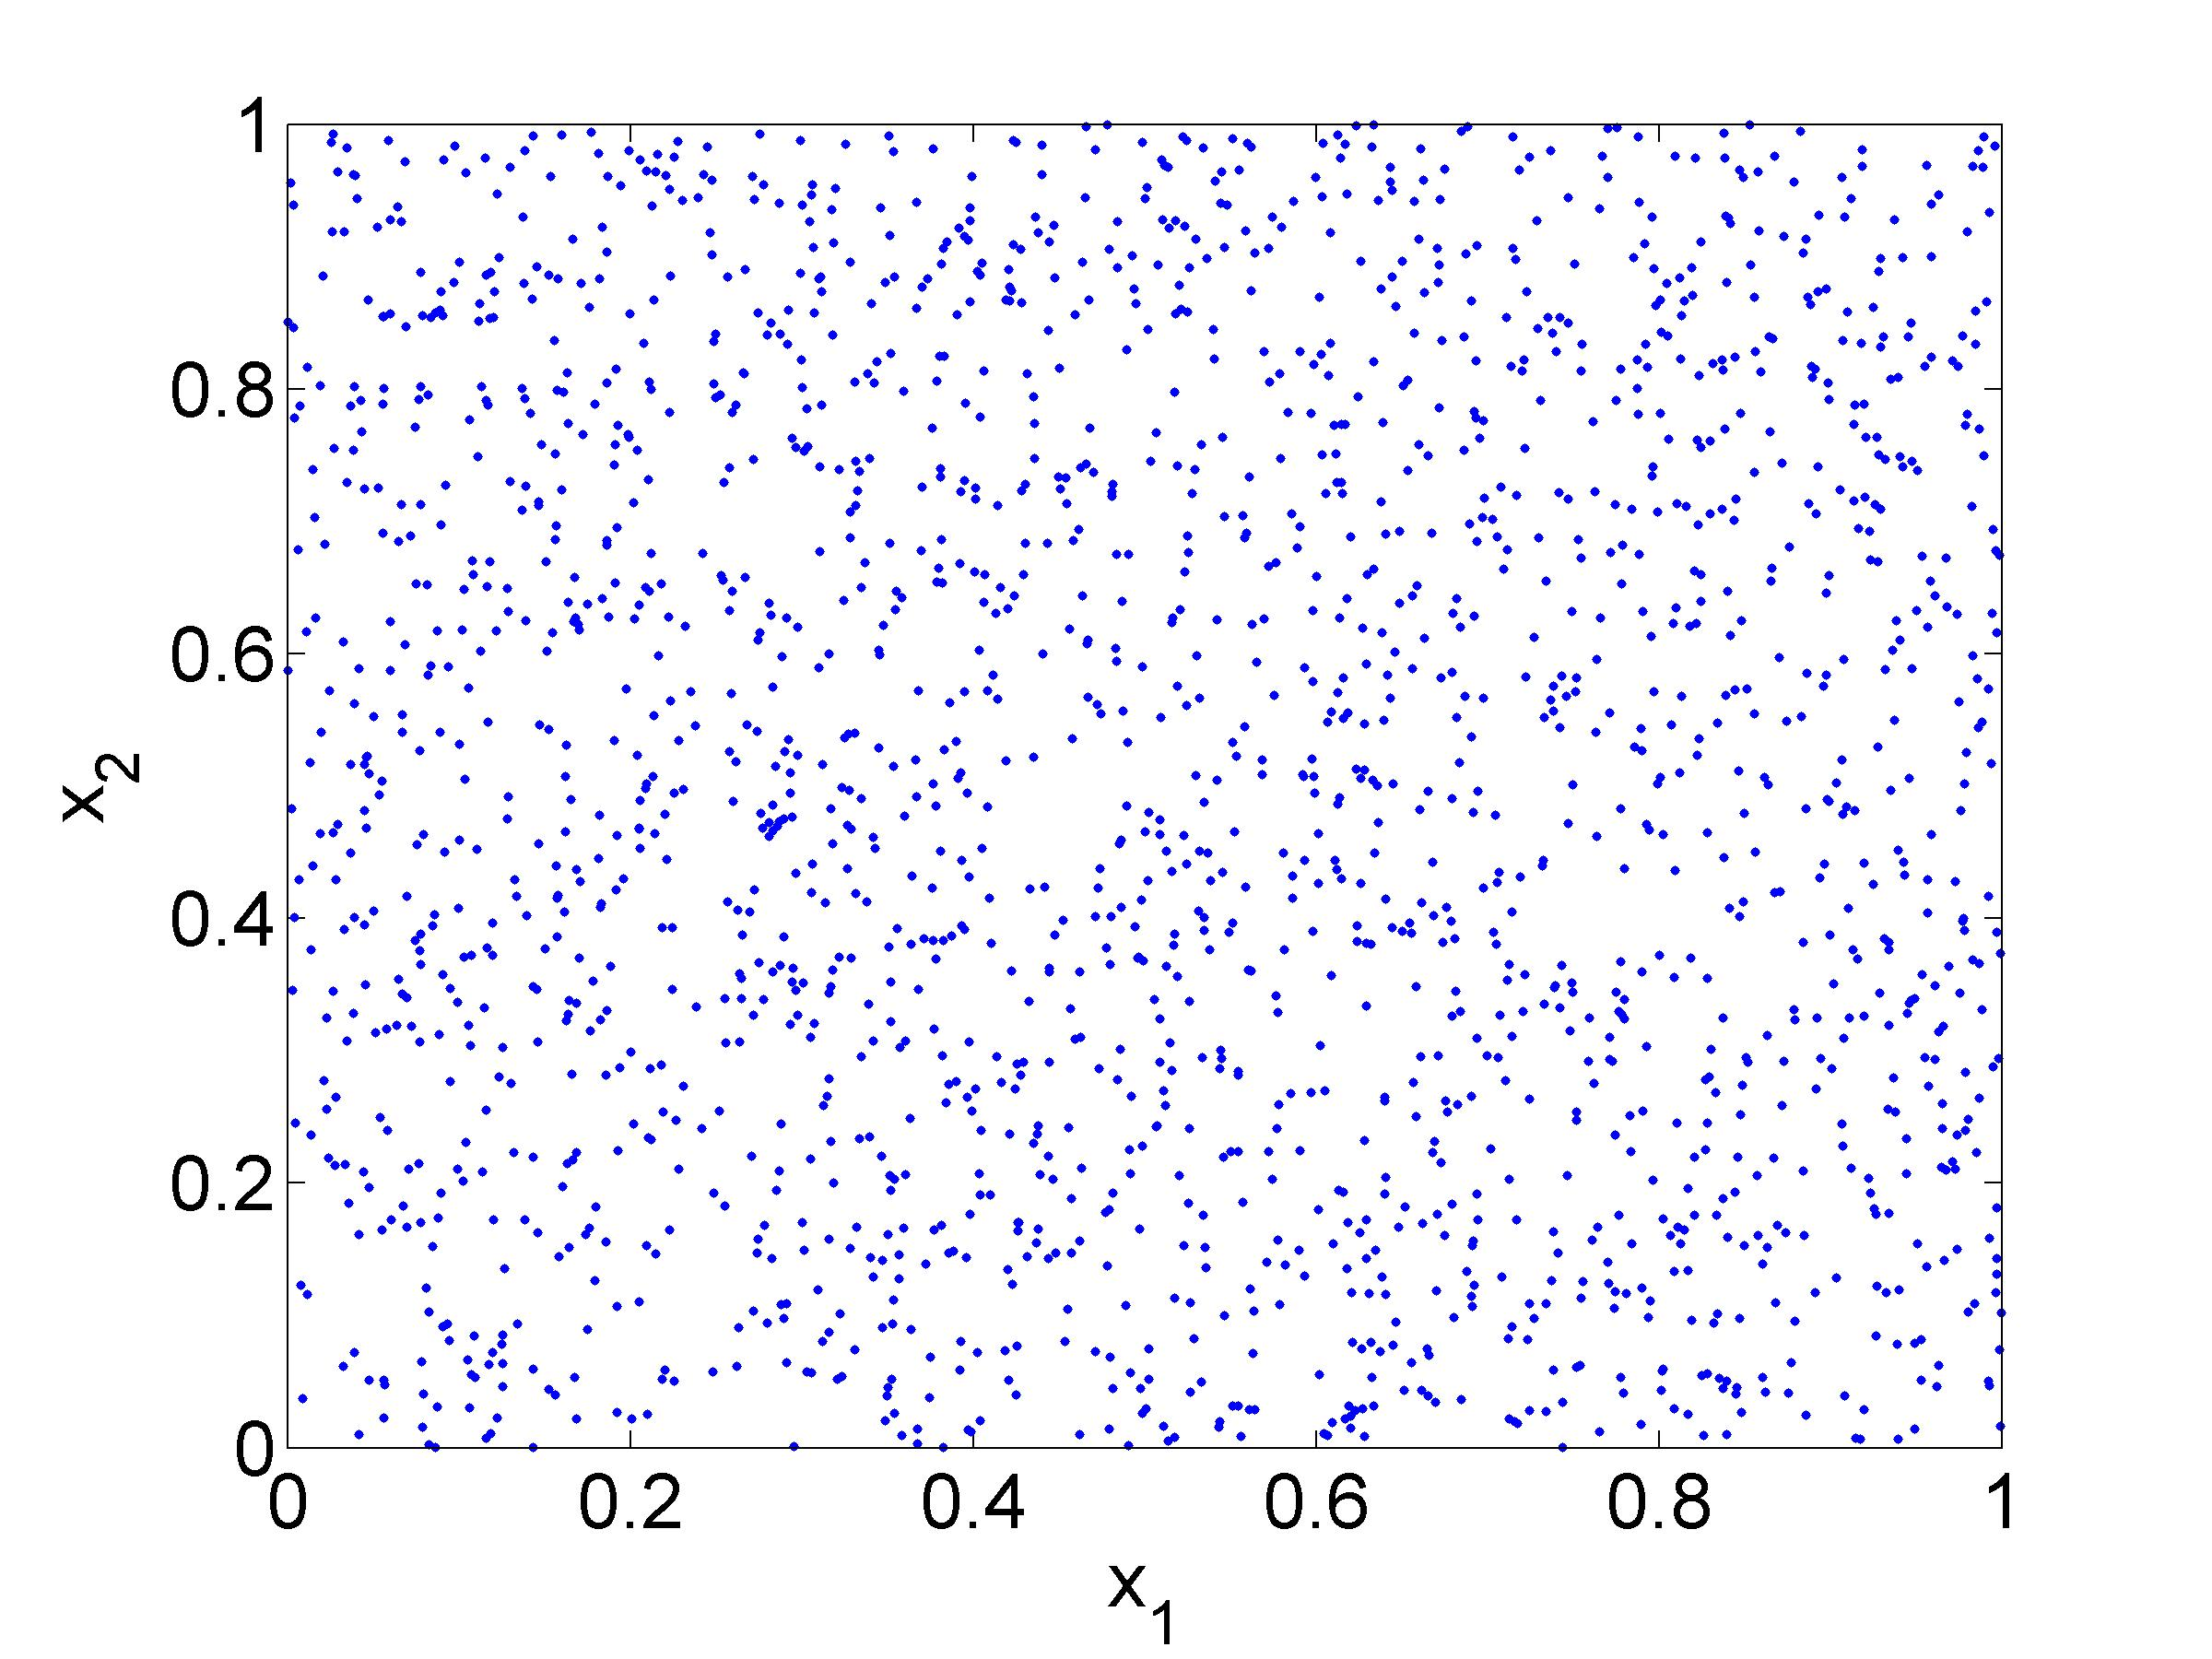
\includegraphics[width=0.5\textwidth]{xdata}
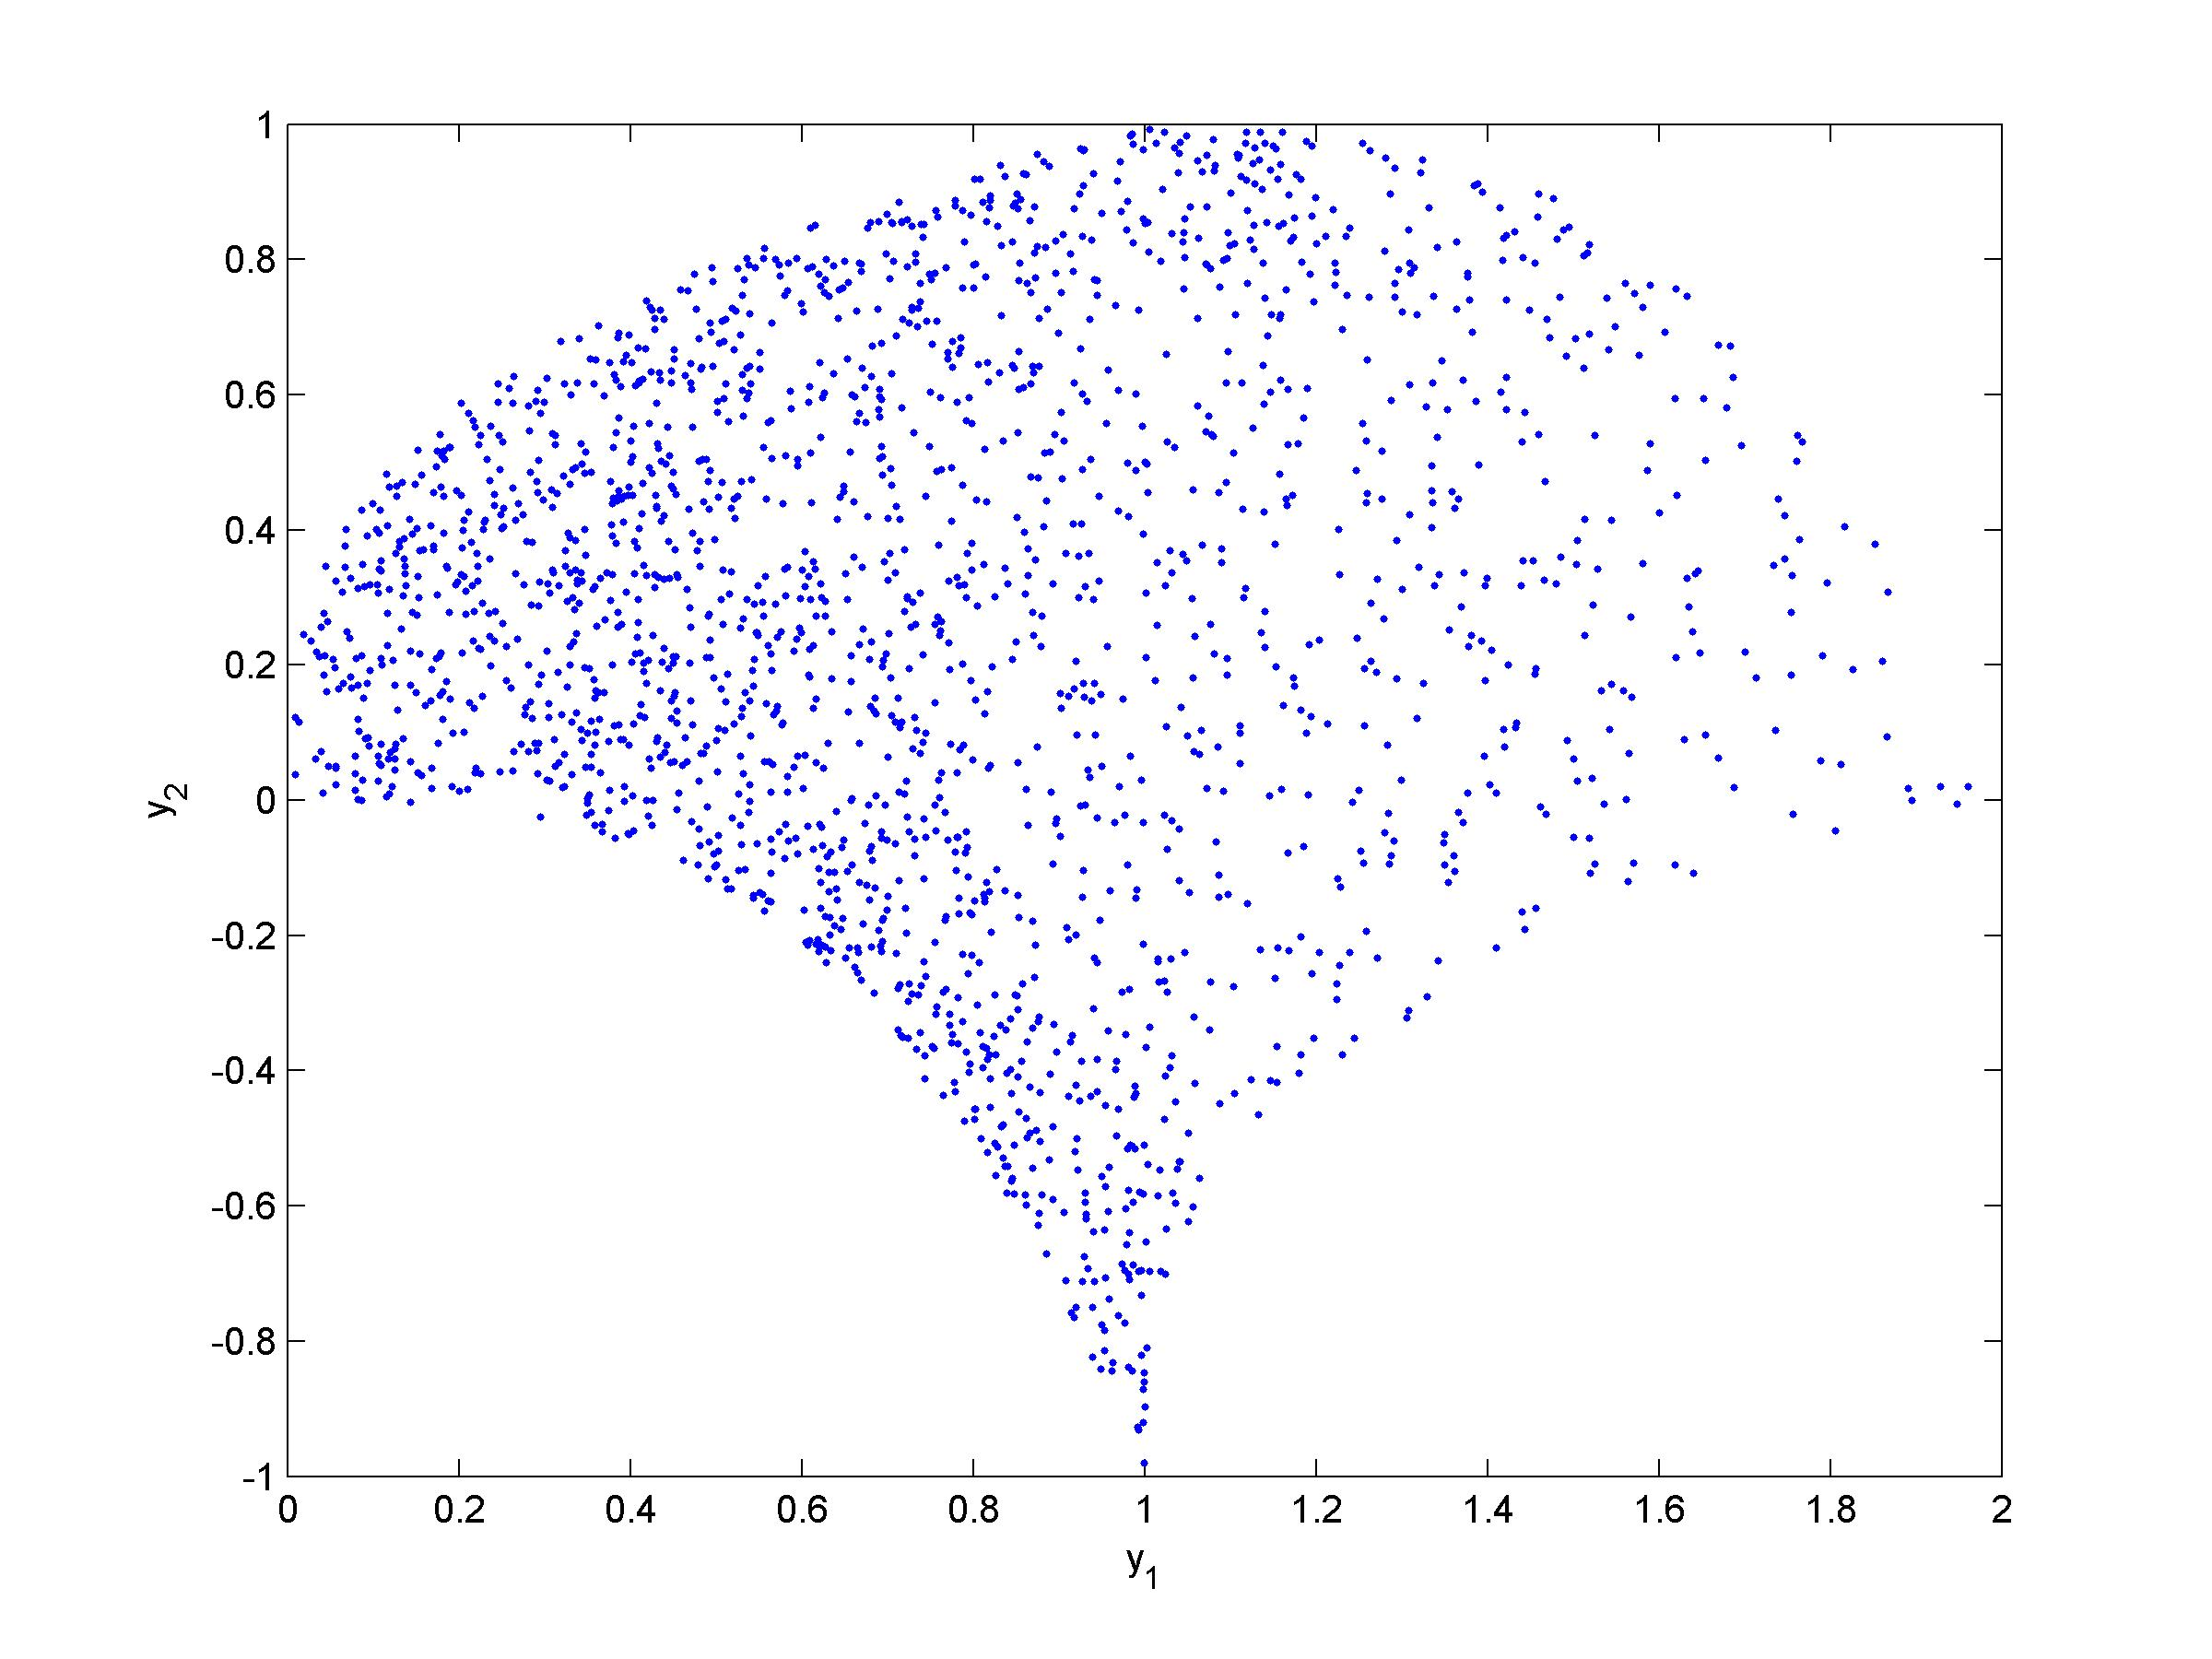
\includegraphics[width=0.5\textwidth]{ydata}
\caption{Left: data in ``true'' space. Right: data in ``ambient'' space.}
\label{fig:data}
\end{figure}

The results of doing DMAPS with the data $y_1, y_2$ are shown in in Figure \ref{fig:xdata_dmaps}.
%
Note that we do not recover the ``correct'' parameterization of the underlying variables $x_1, x_2$.

\begin{figure}[htb]
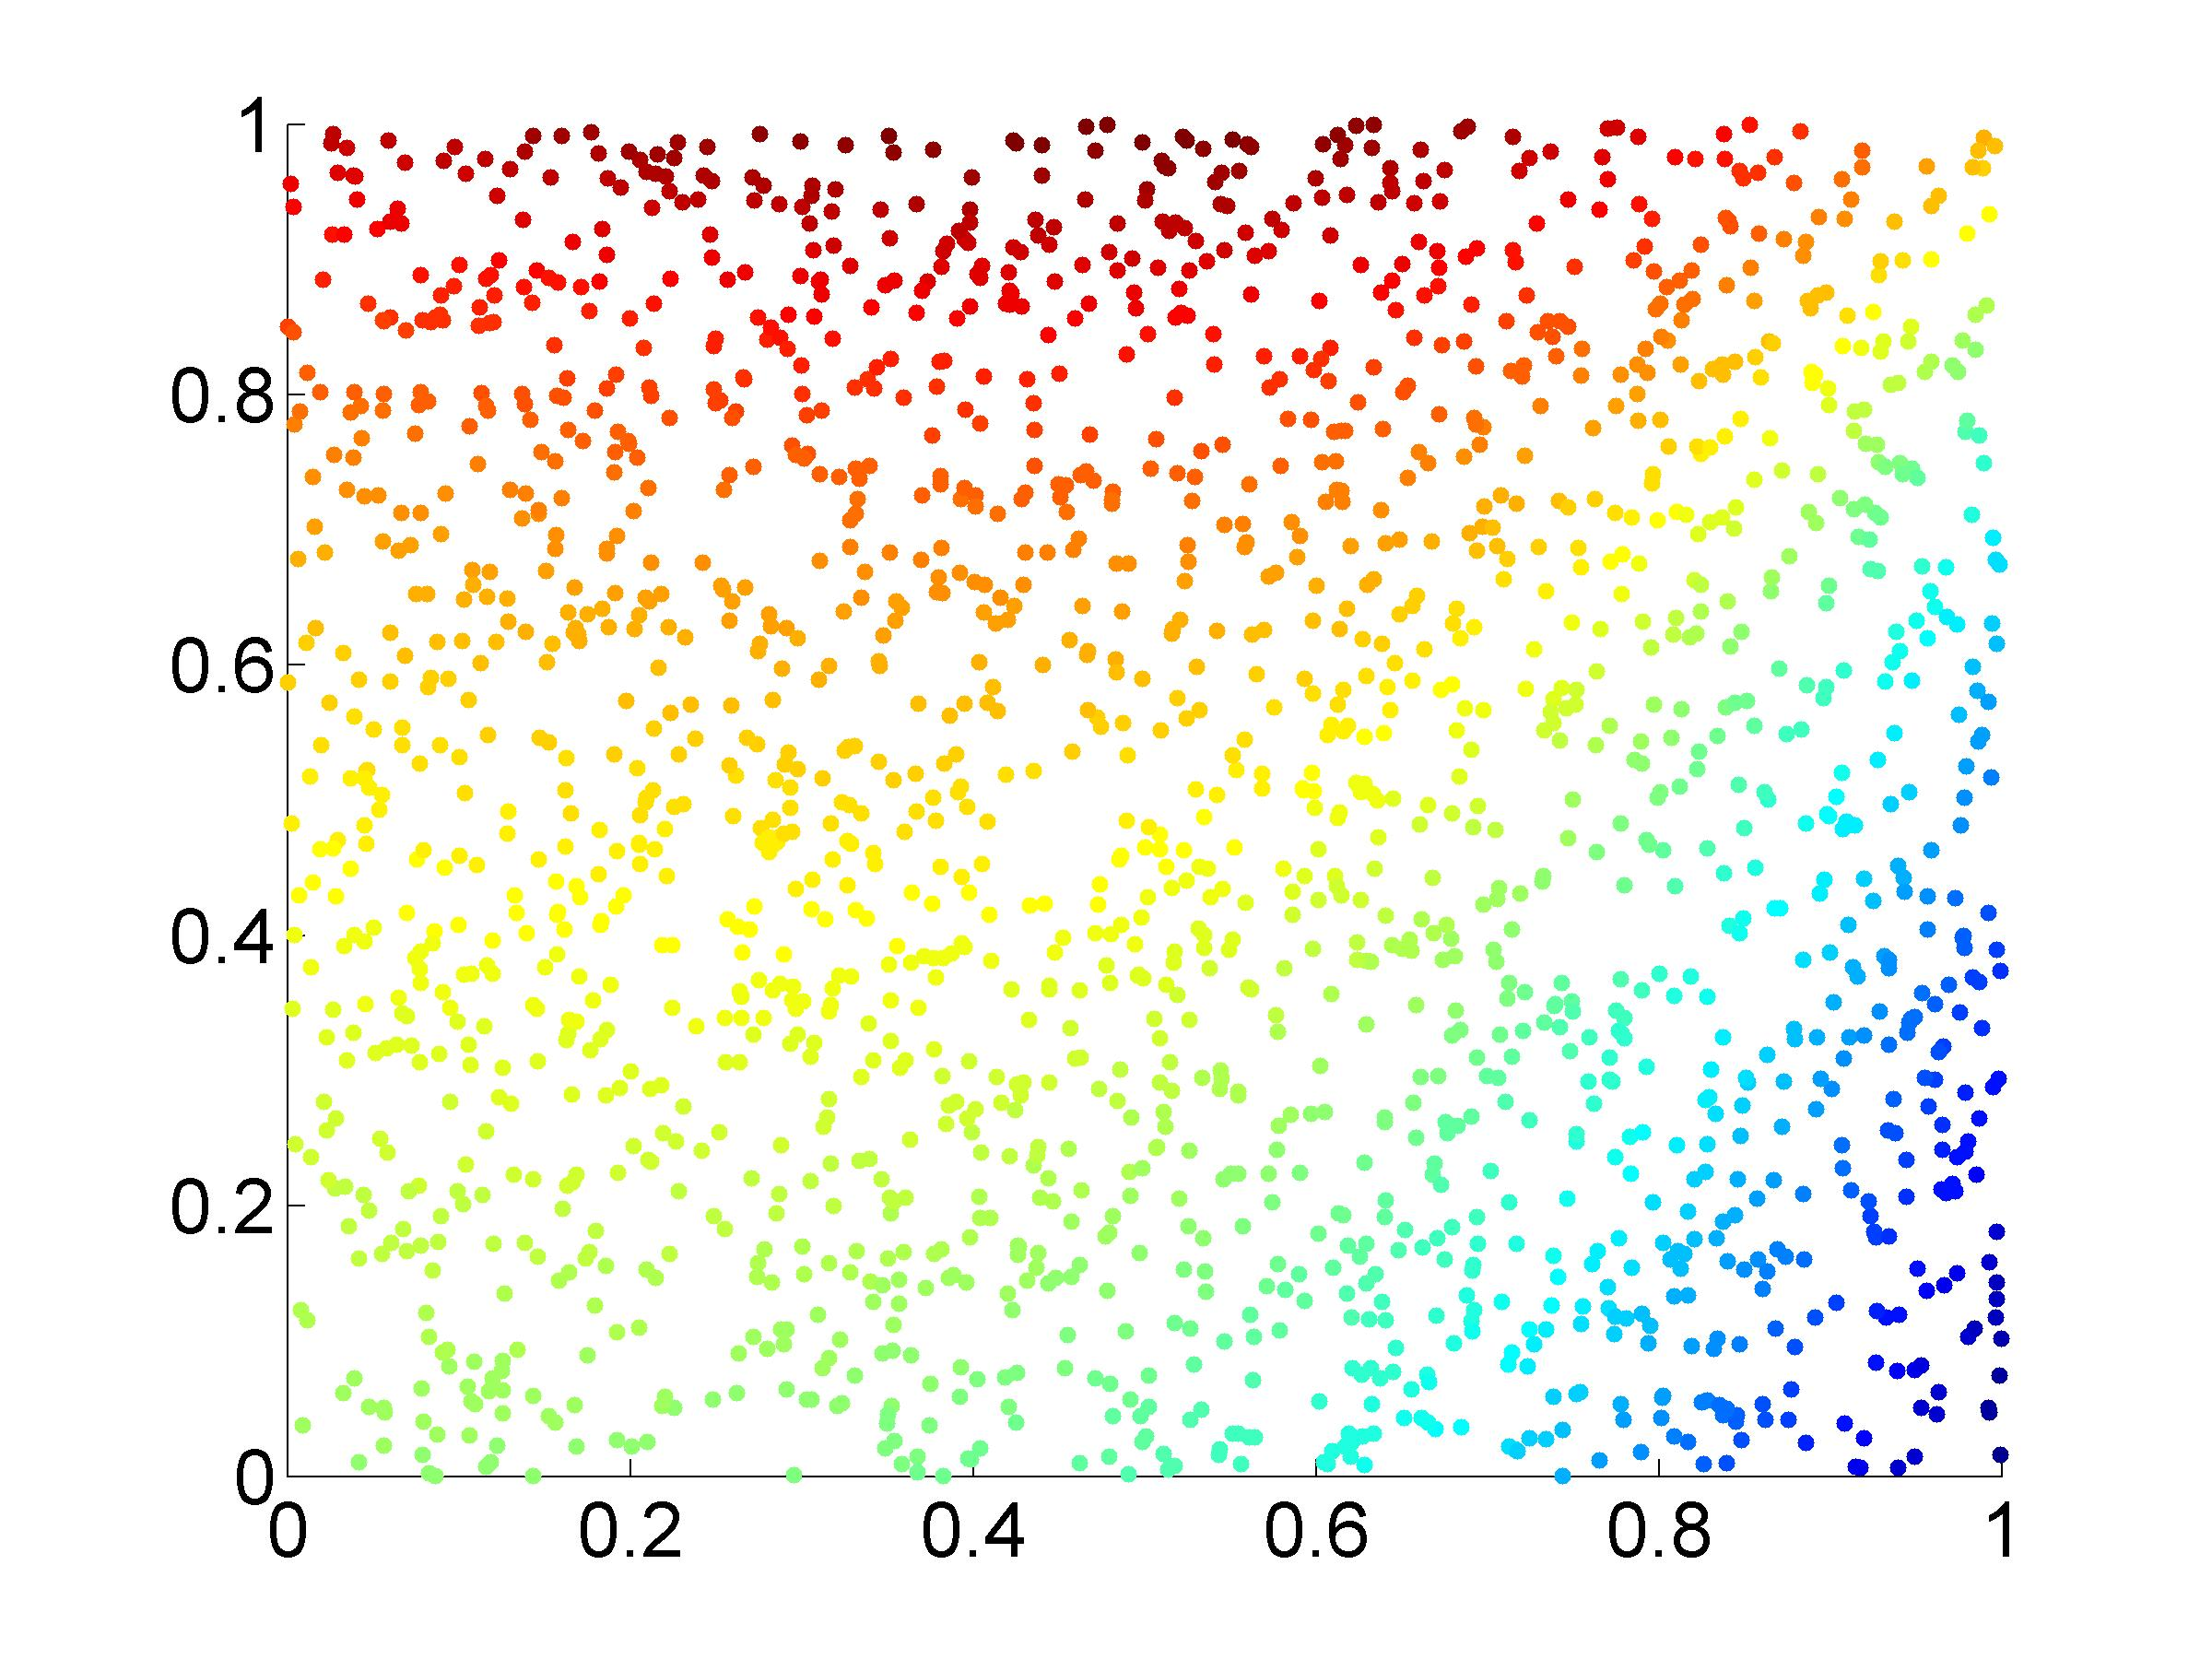
\includegraphics[width=0.3\textwidth]{xdata_colored_DMAPS1}
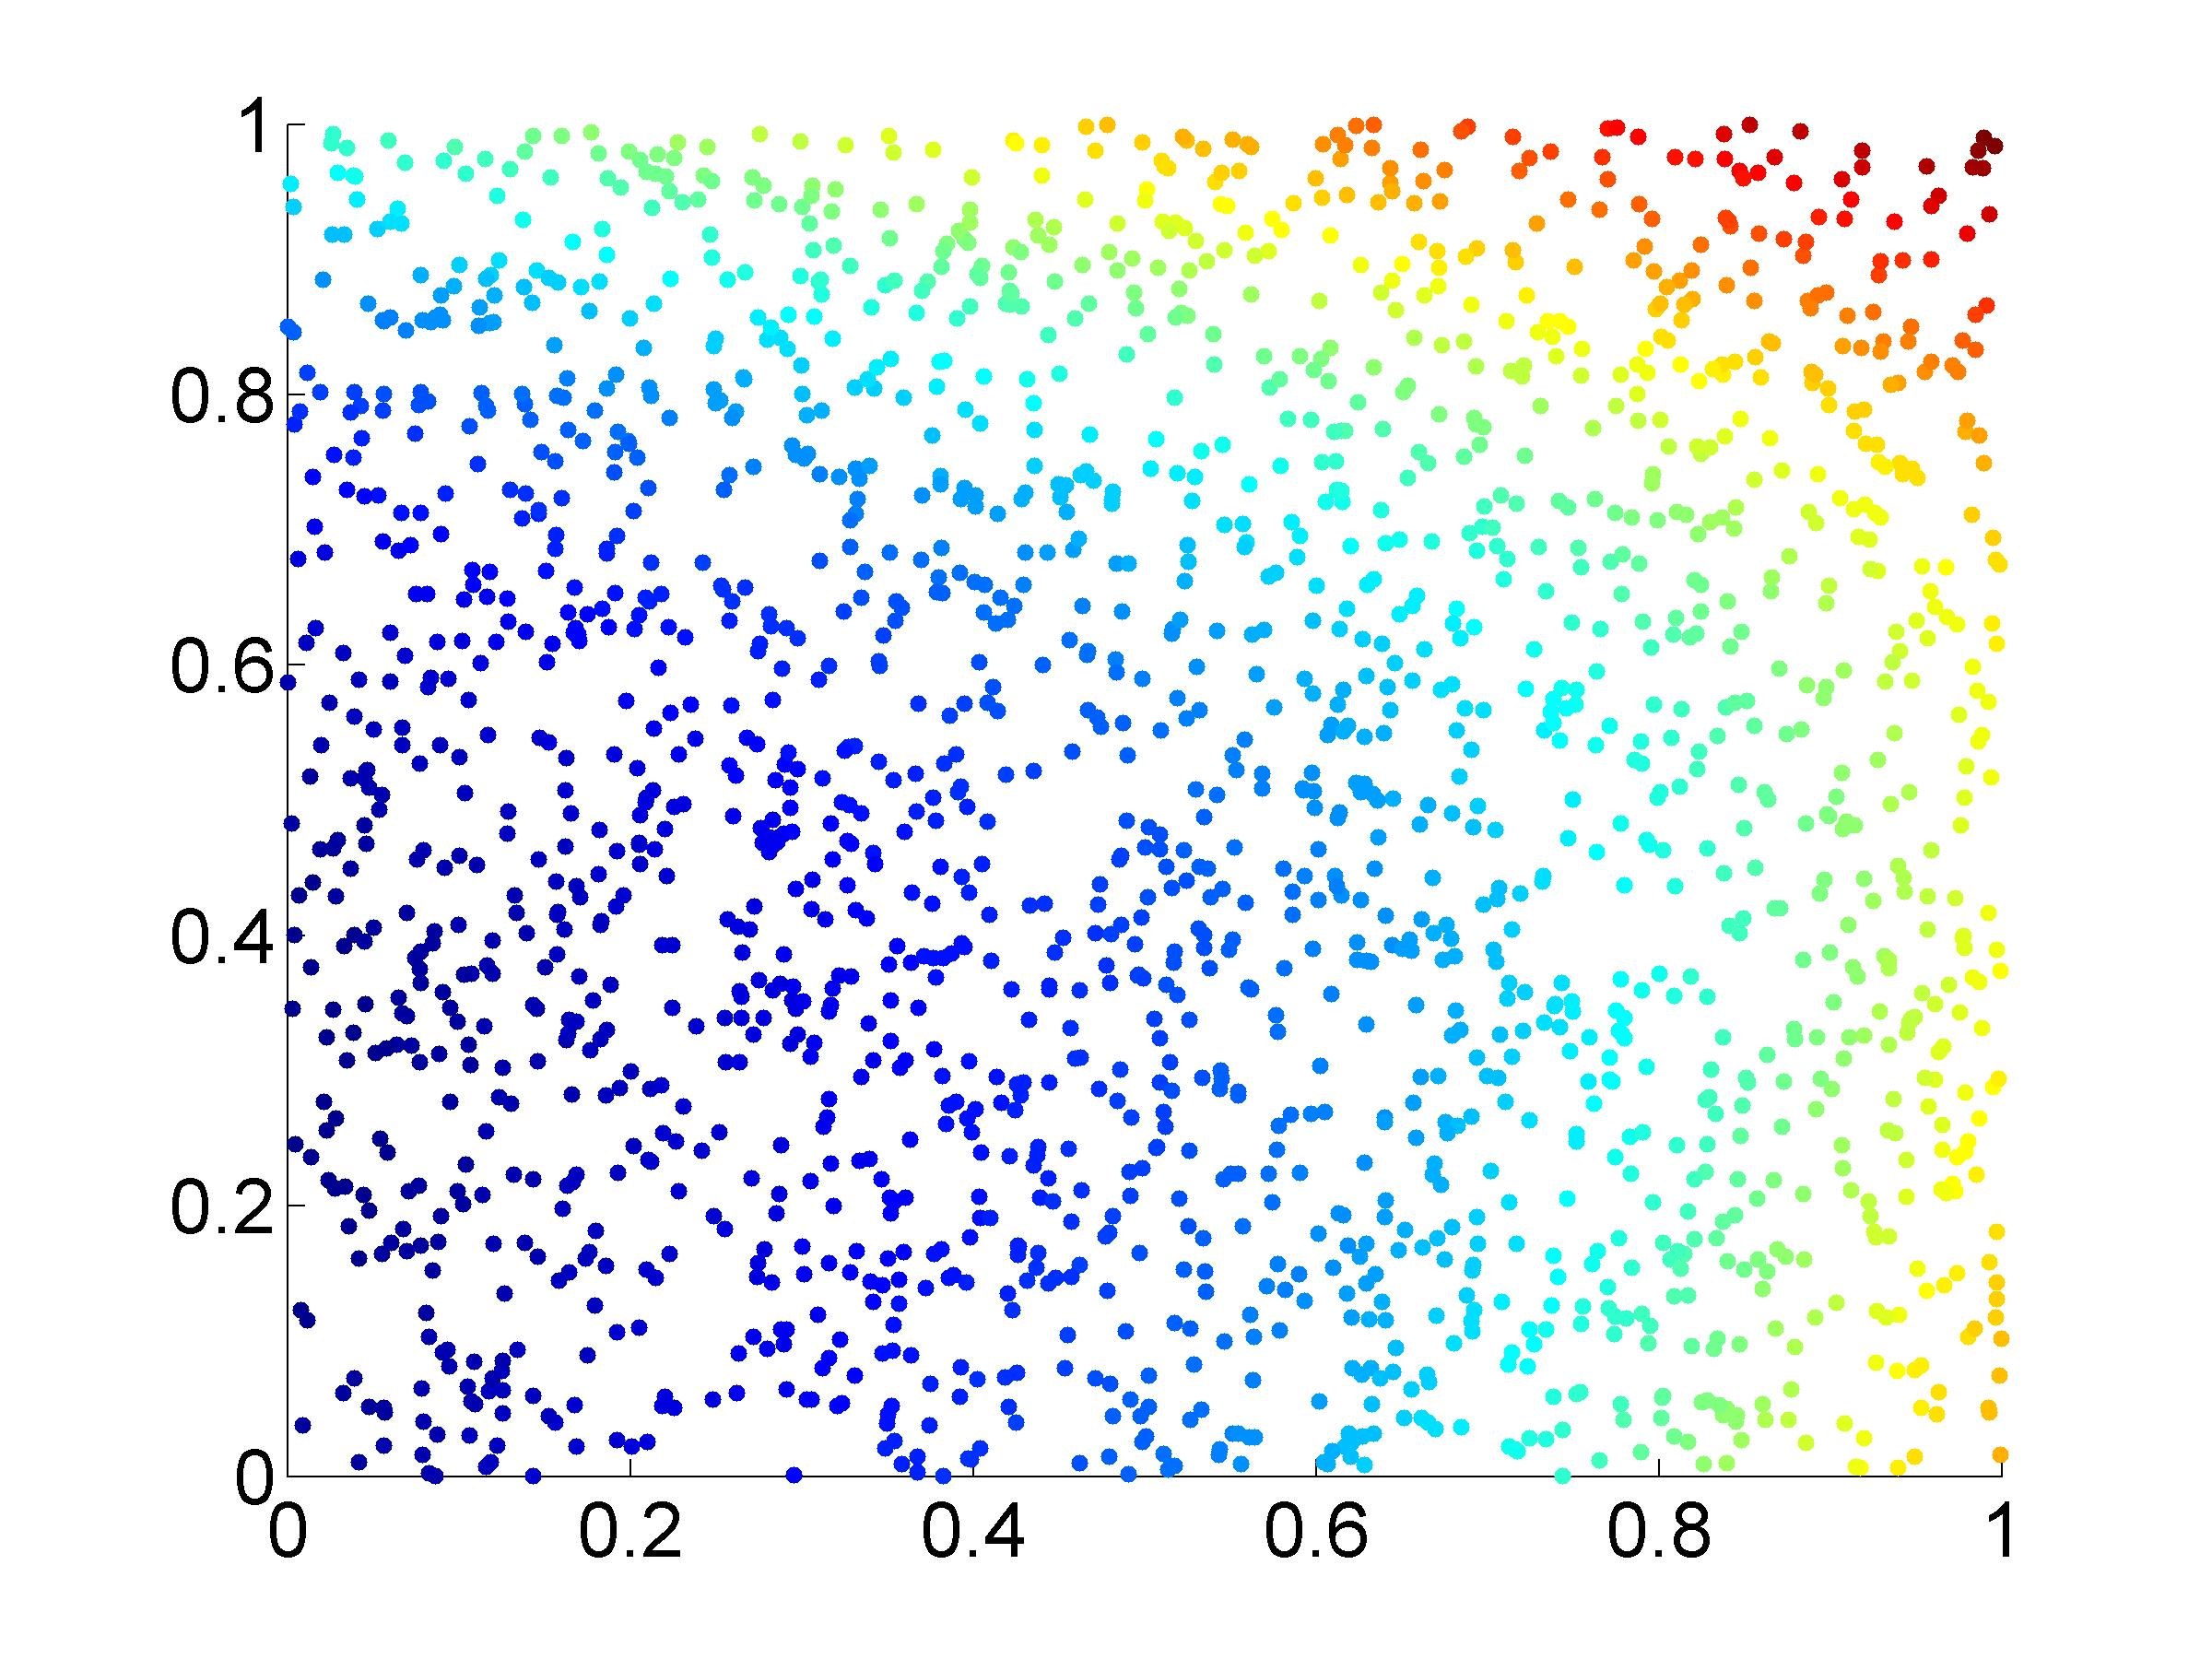
\includegraphics[width=0.3\textwidth]{xdata_colored_DMAPS2}
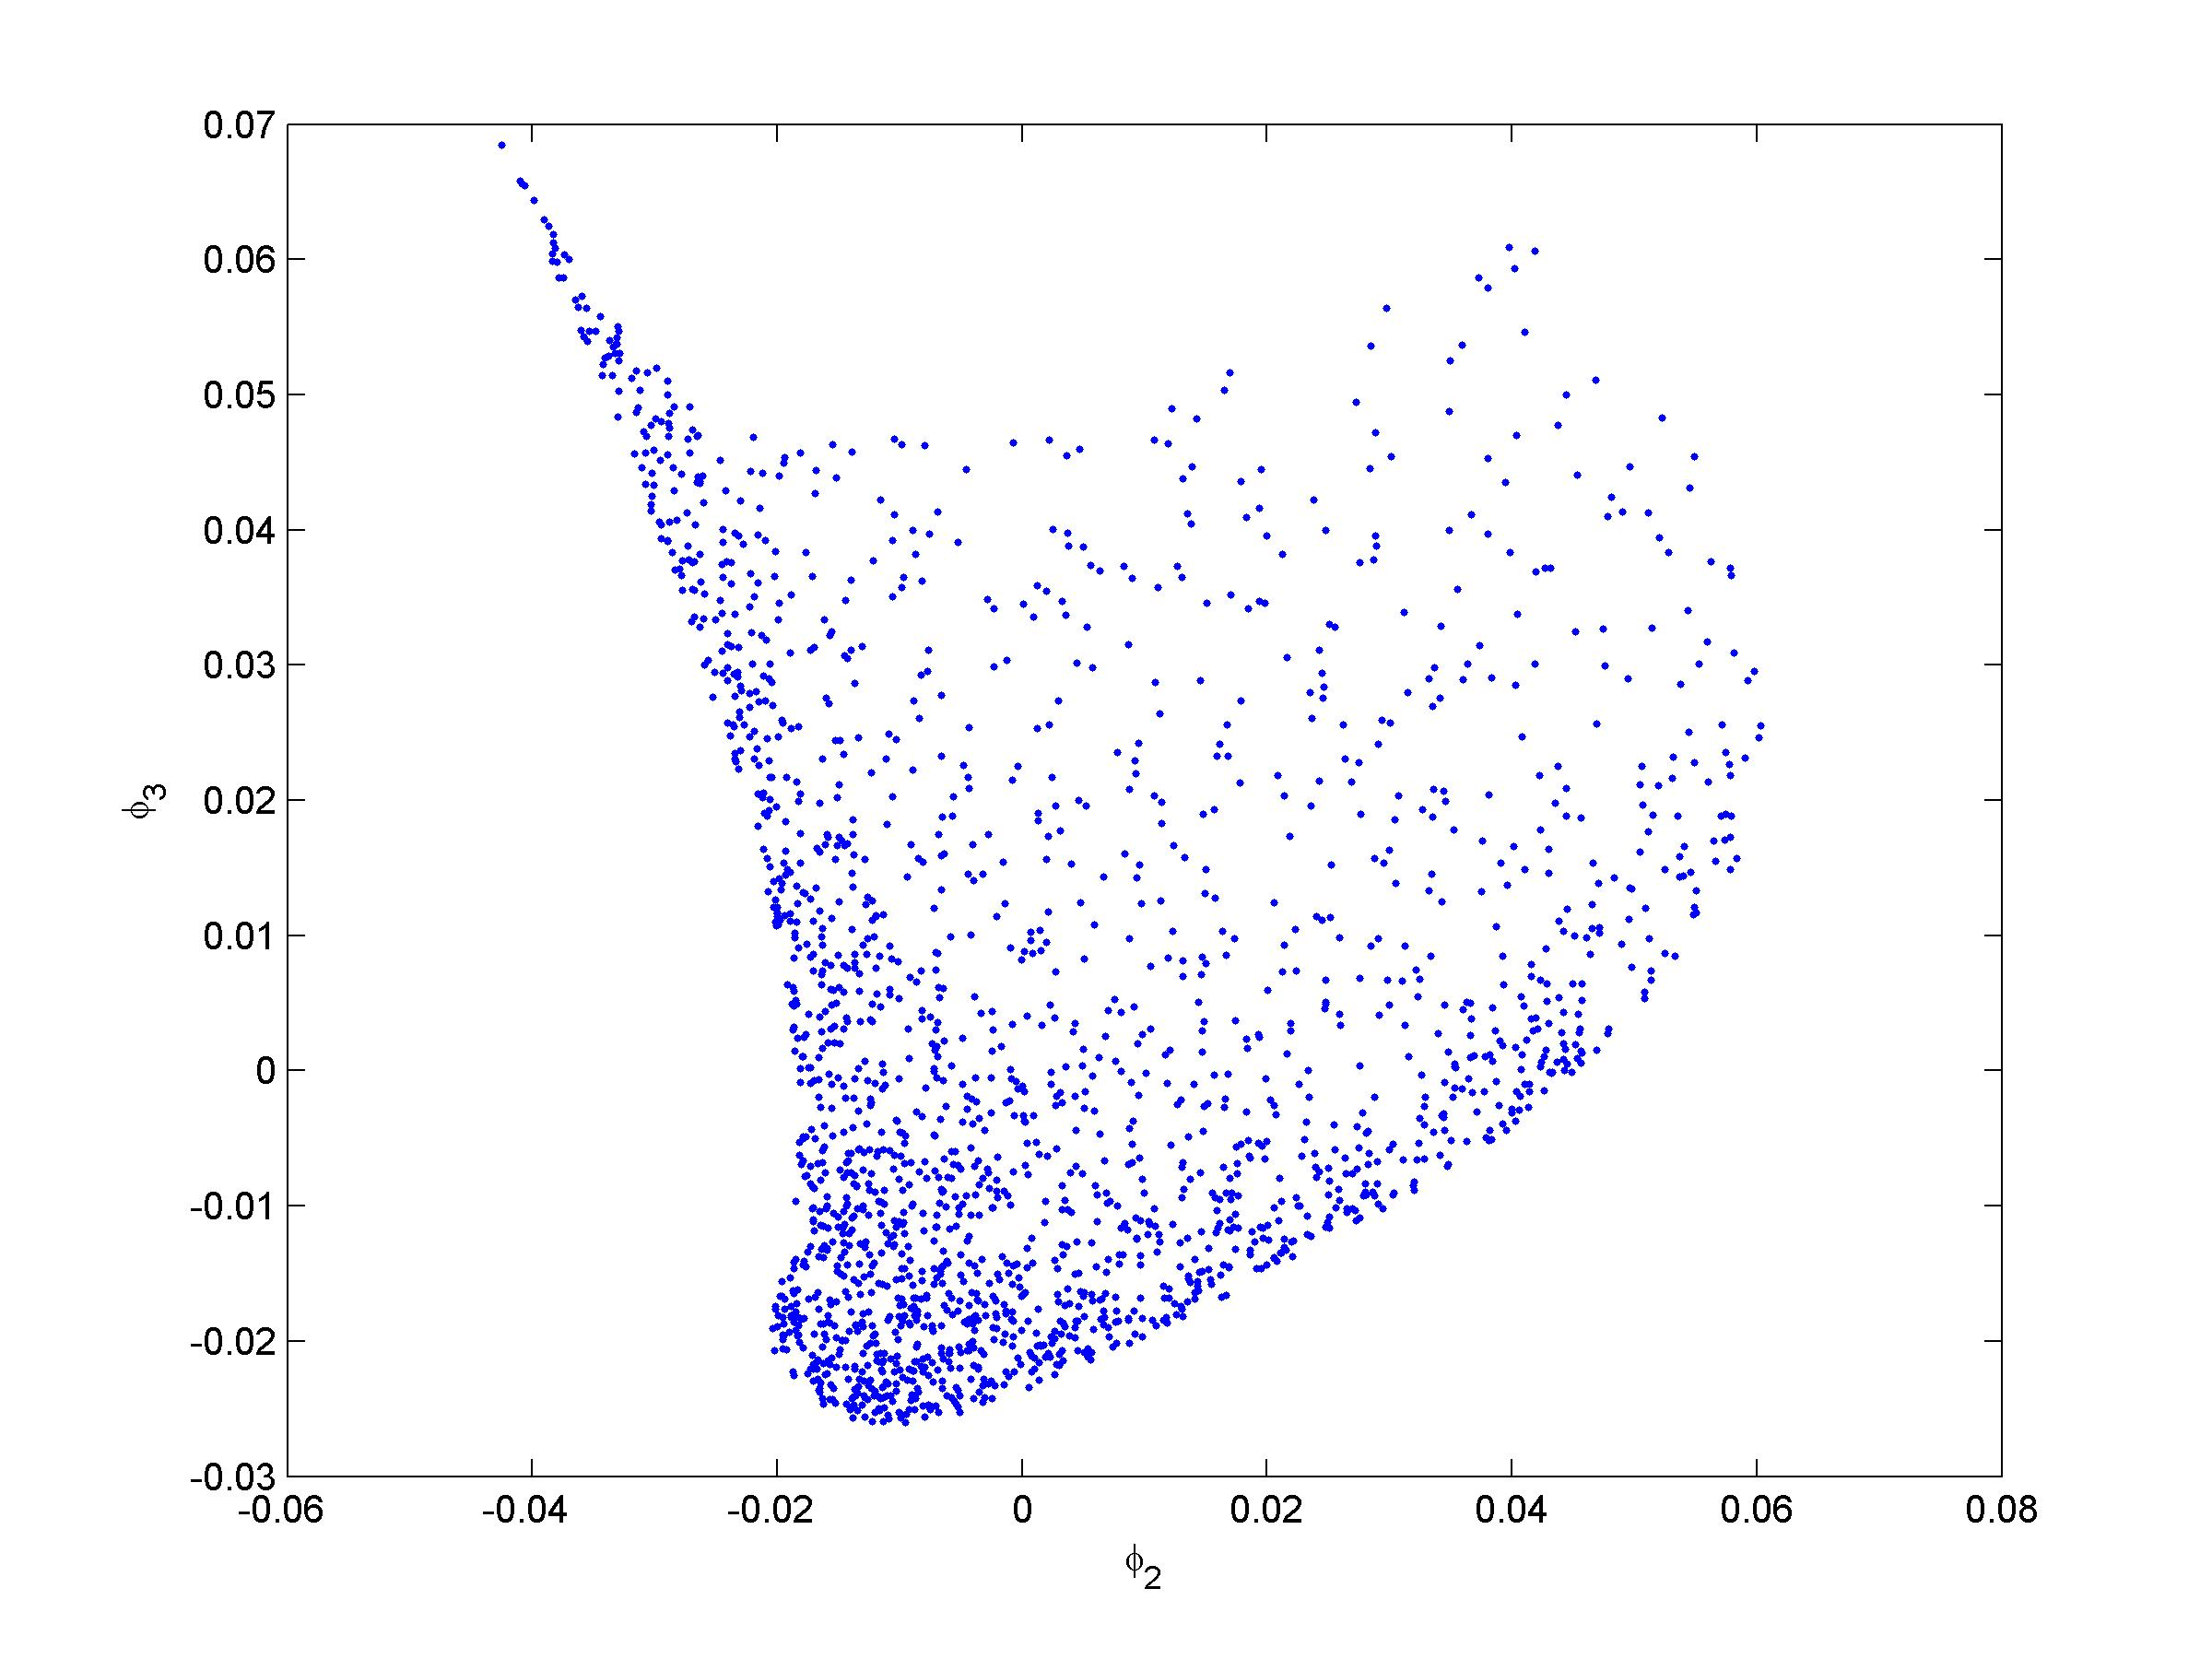
\includegraphics[width=0.3\textwidth]{embedding_dmaps}
\caption{Data in ``true'' space ($x_1, x_2$), colored by the first (left) and second (center) nontrivial DMAPS component. The DMAPS embedding is computed from the data in the ``ambient'' space ($y_1, y_2$). Note that the parameterizationa we obtain are not the eigenfunctions that we expect for points sampled from the unit square. (Right) Data plotted in first two (nontrivial) DMAPS variables.}
\label{fig:xdata_dmaps}
\end{figure}

If we do NIV with the data $y_1, y_2$, 
%taking our time windows so that the clouds around the points have standard deviation $1e-3$, 
we obtain the results in Figure \ref{fig:xdata_NIV}.
%
Note that we now recover the ``correct'' variables.

\begin{figure}[htb]
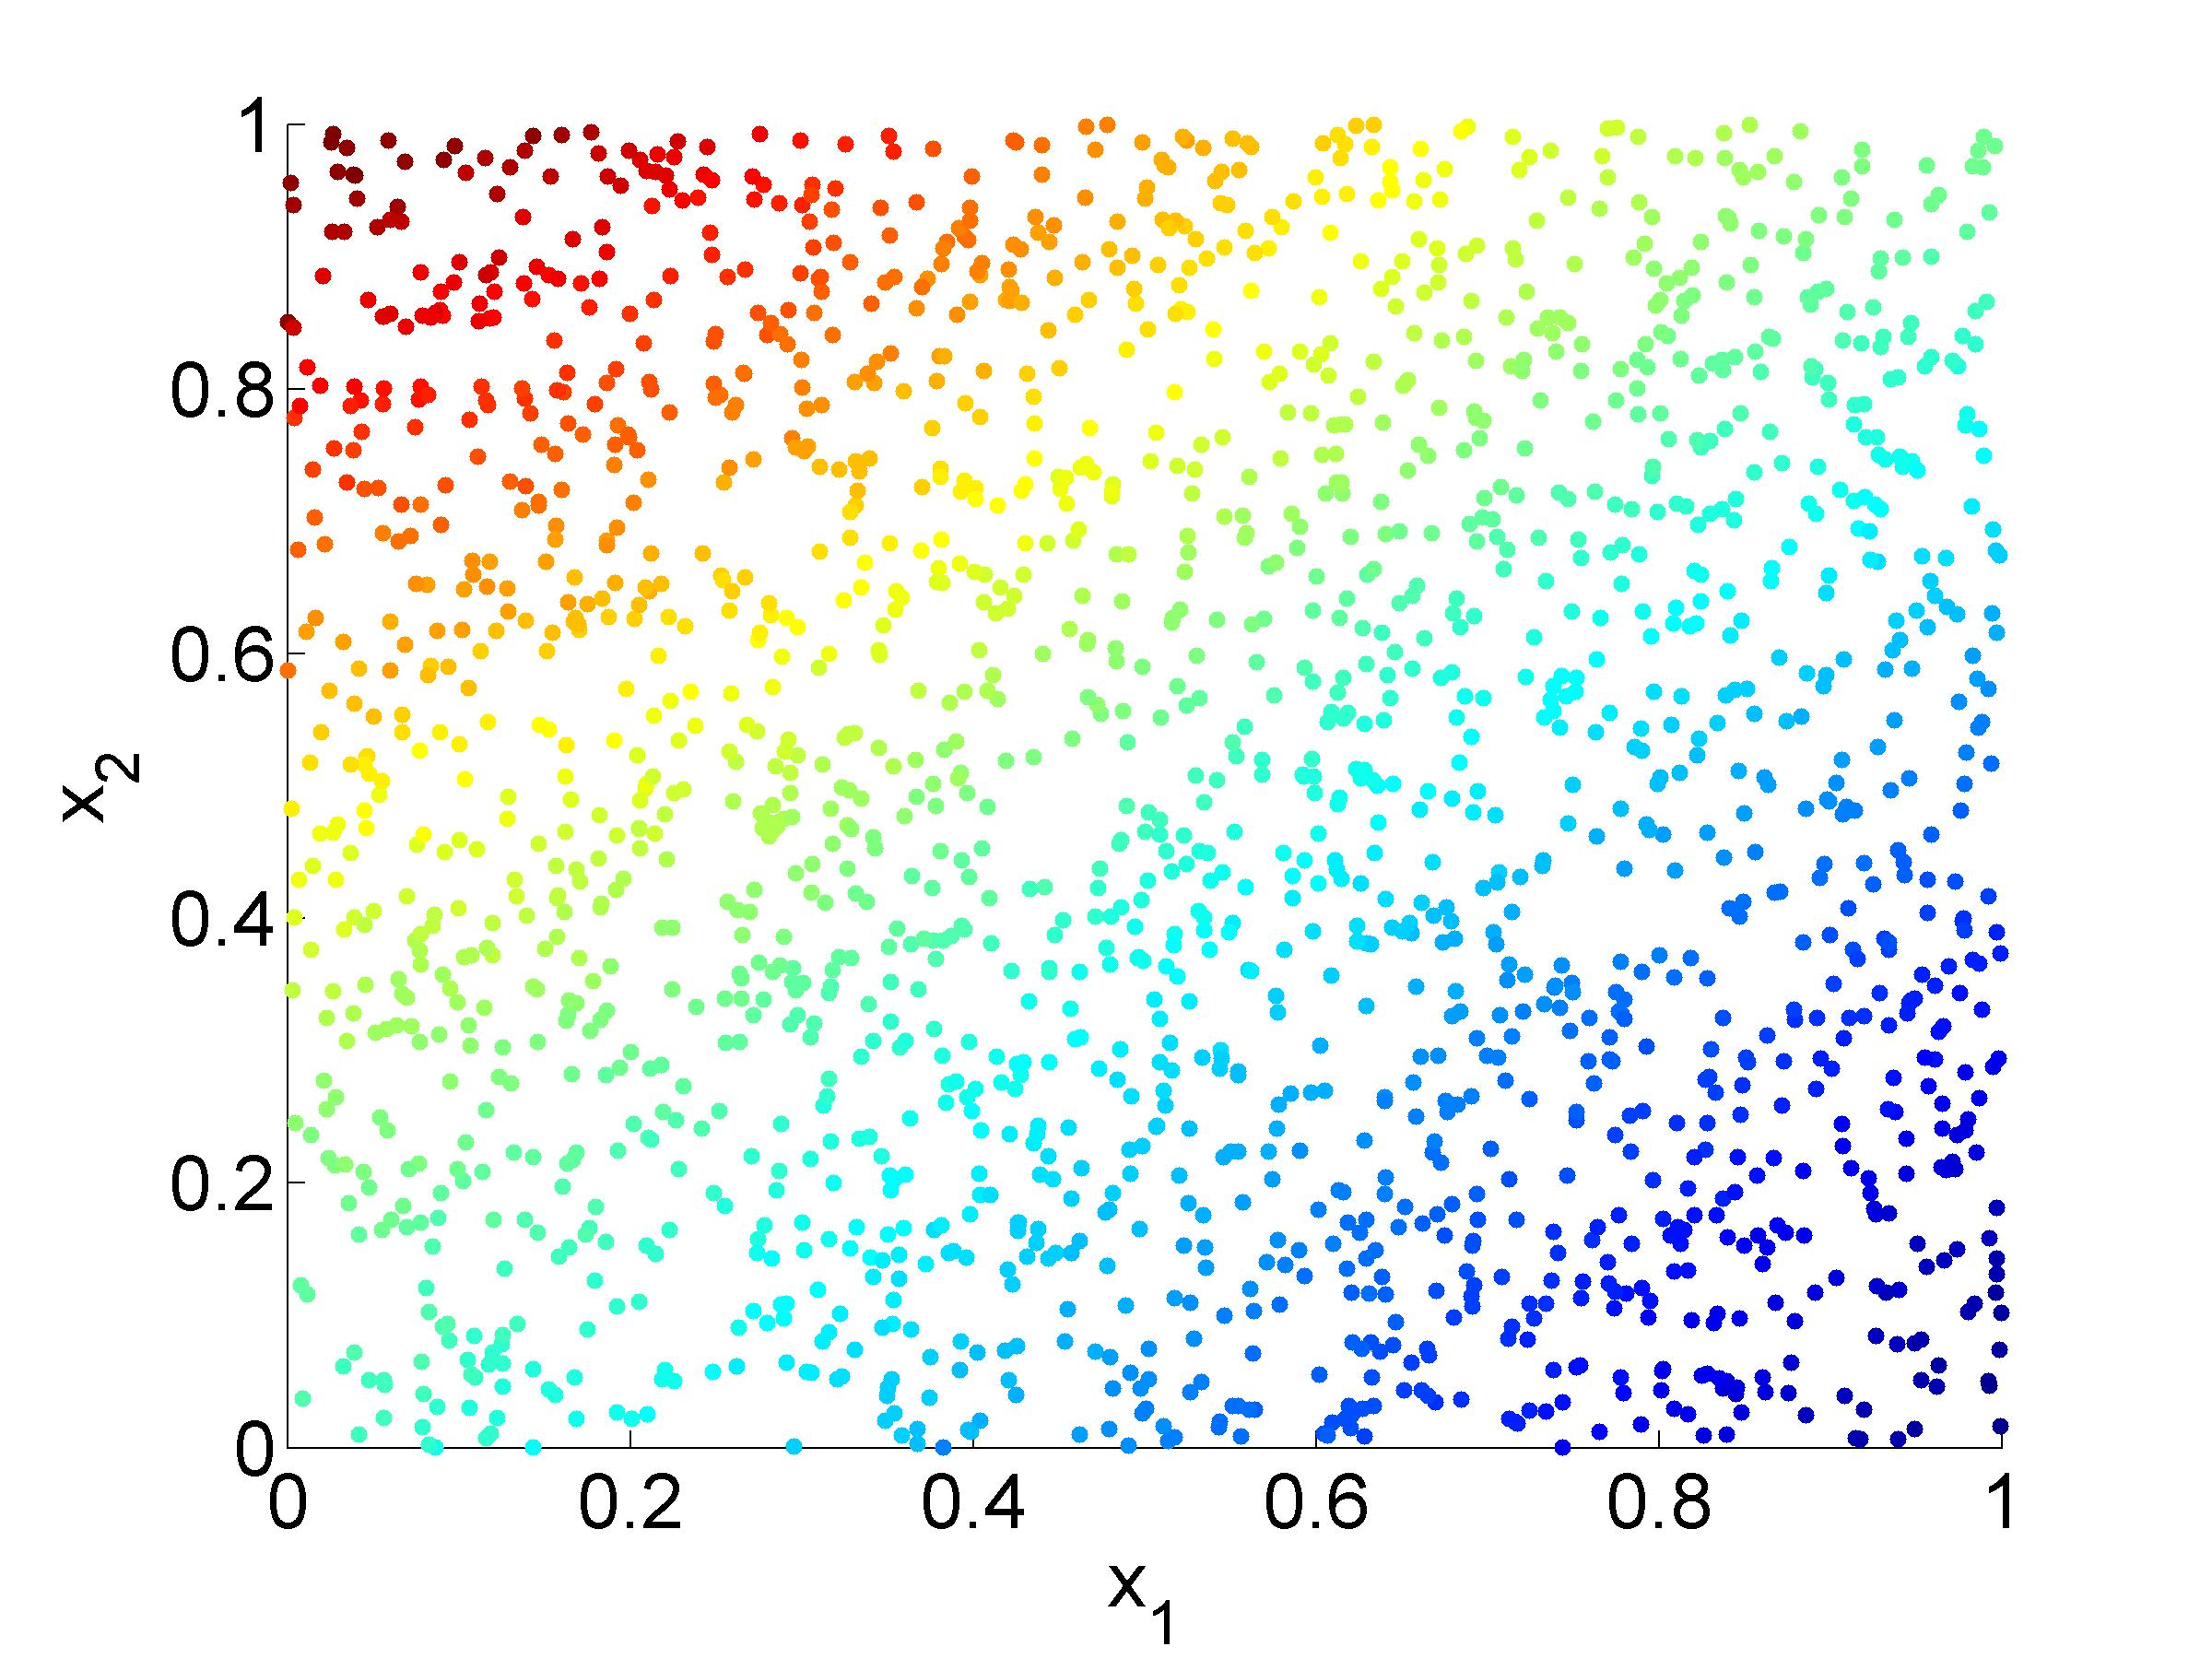
\includegraphics[width=0.3\textwidth]{xdata_colored_NIV1}
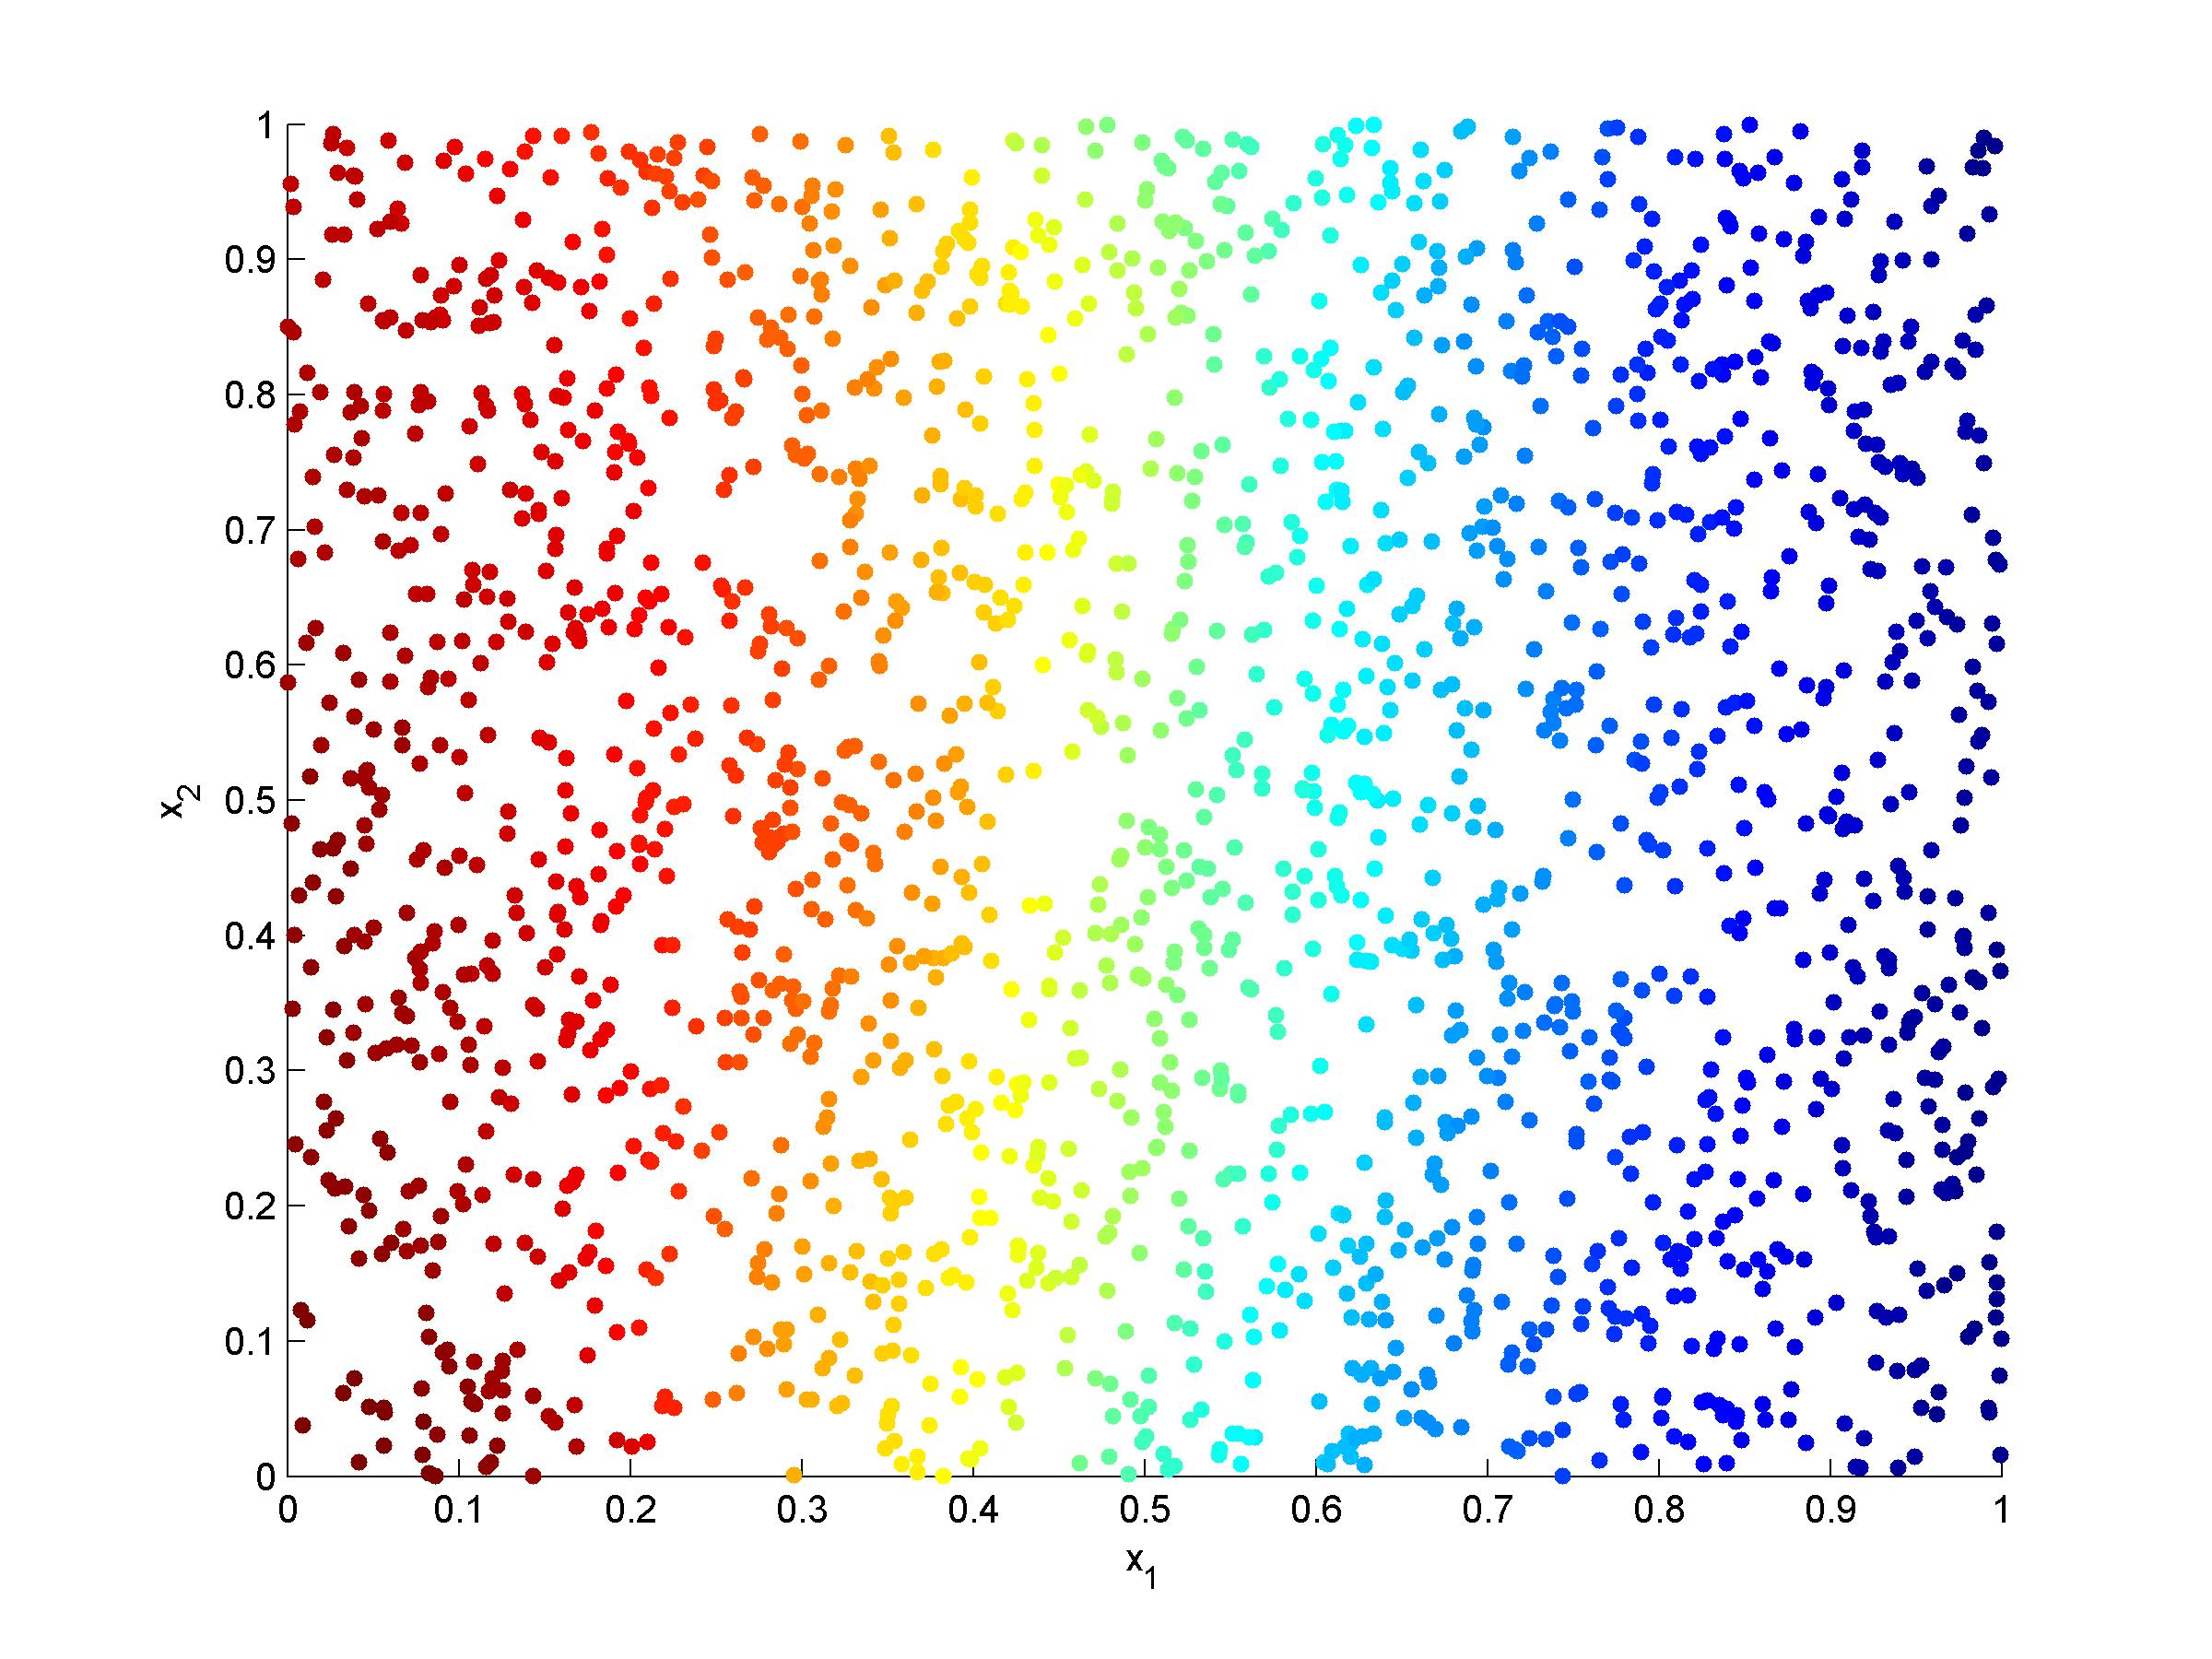
\includegraphics[width=0.3\textwidth]{xdata_colored_NIV2}
\includegraphics[width=0.3\textwidth]{embedding_NIV}
\caption{Data in ``true'' space ($x_1, x_2$), colored by the first (left) and second (center) nontrivial NIV. The NIV embedding is computed from the data in the ambient space ($y_1, y_2$), with time window $\Delta t = 0.01$. Note that the parameterizations we obtain are the eigenfunctions that we expect for points sampled from the unit square. (Right) Data plotted in first two (nontrivial) NIV.}
\label{fig:xdata_NIV}
\end{figure}

We now look at the effect of adding additional noise to our system.
%
Consider adding white Gaussian noise to the $y_1, y_2$ data
\begin{eqnarray}
z_1 & = & x_1 + x_2^3 + \xi_1 \\
z_2 & = & x_2 - x_1^3 + \xi_2 \\
z_3 & = & \xi_3
\end{eqnarray}
where $\xi_1, \xi_2, \xi_3 \sim \mathcal{N}(0, \sigma^2)$

If $\sigma = 0.01$ (so the added noise is much smaller than the noise in the original clouds), we obtain a parameterization shown in Figure \ref{fig:xdata_NIV_noise1} using NIV.
%
When we do NIV, the ``ellipses'' we see are a combination of the original noises in the intrinsic variables and the noise in the ambient space.
%
Because the noise in the ambient space is significantly smaller than the noise in the original intrinsic variable space, we can still ``see'' the directions of the intrinsic variable noises in the ellipses, and therefore uncover the intrinsic variables.

\begin{figure}[htb]
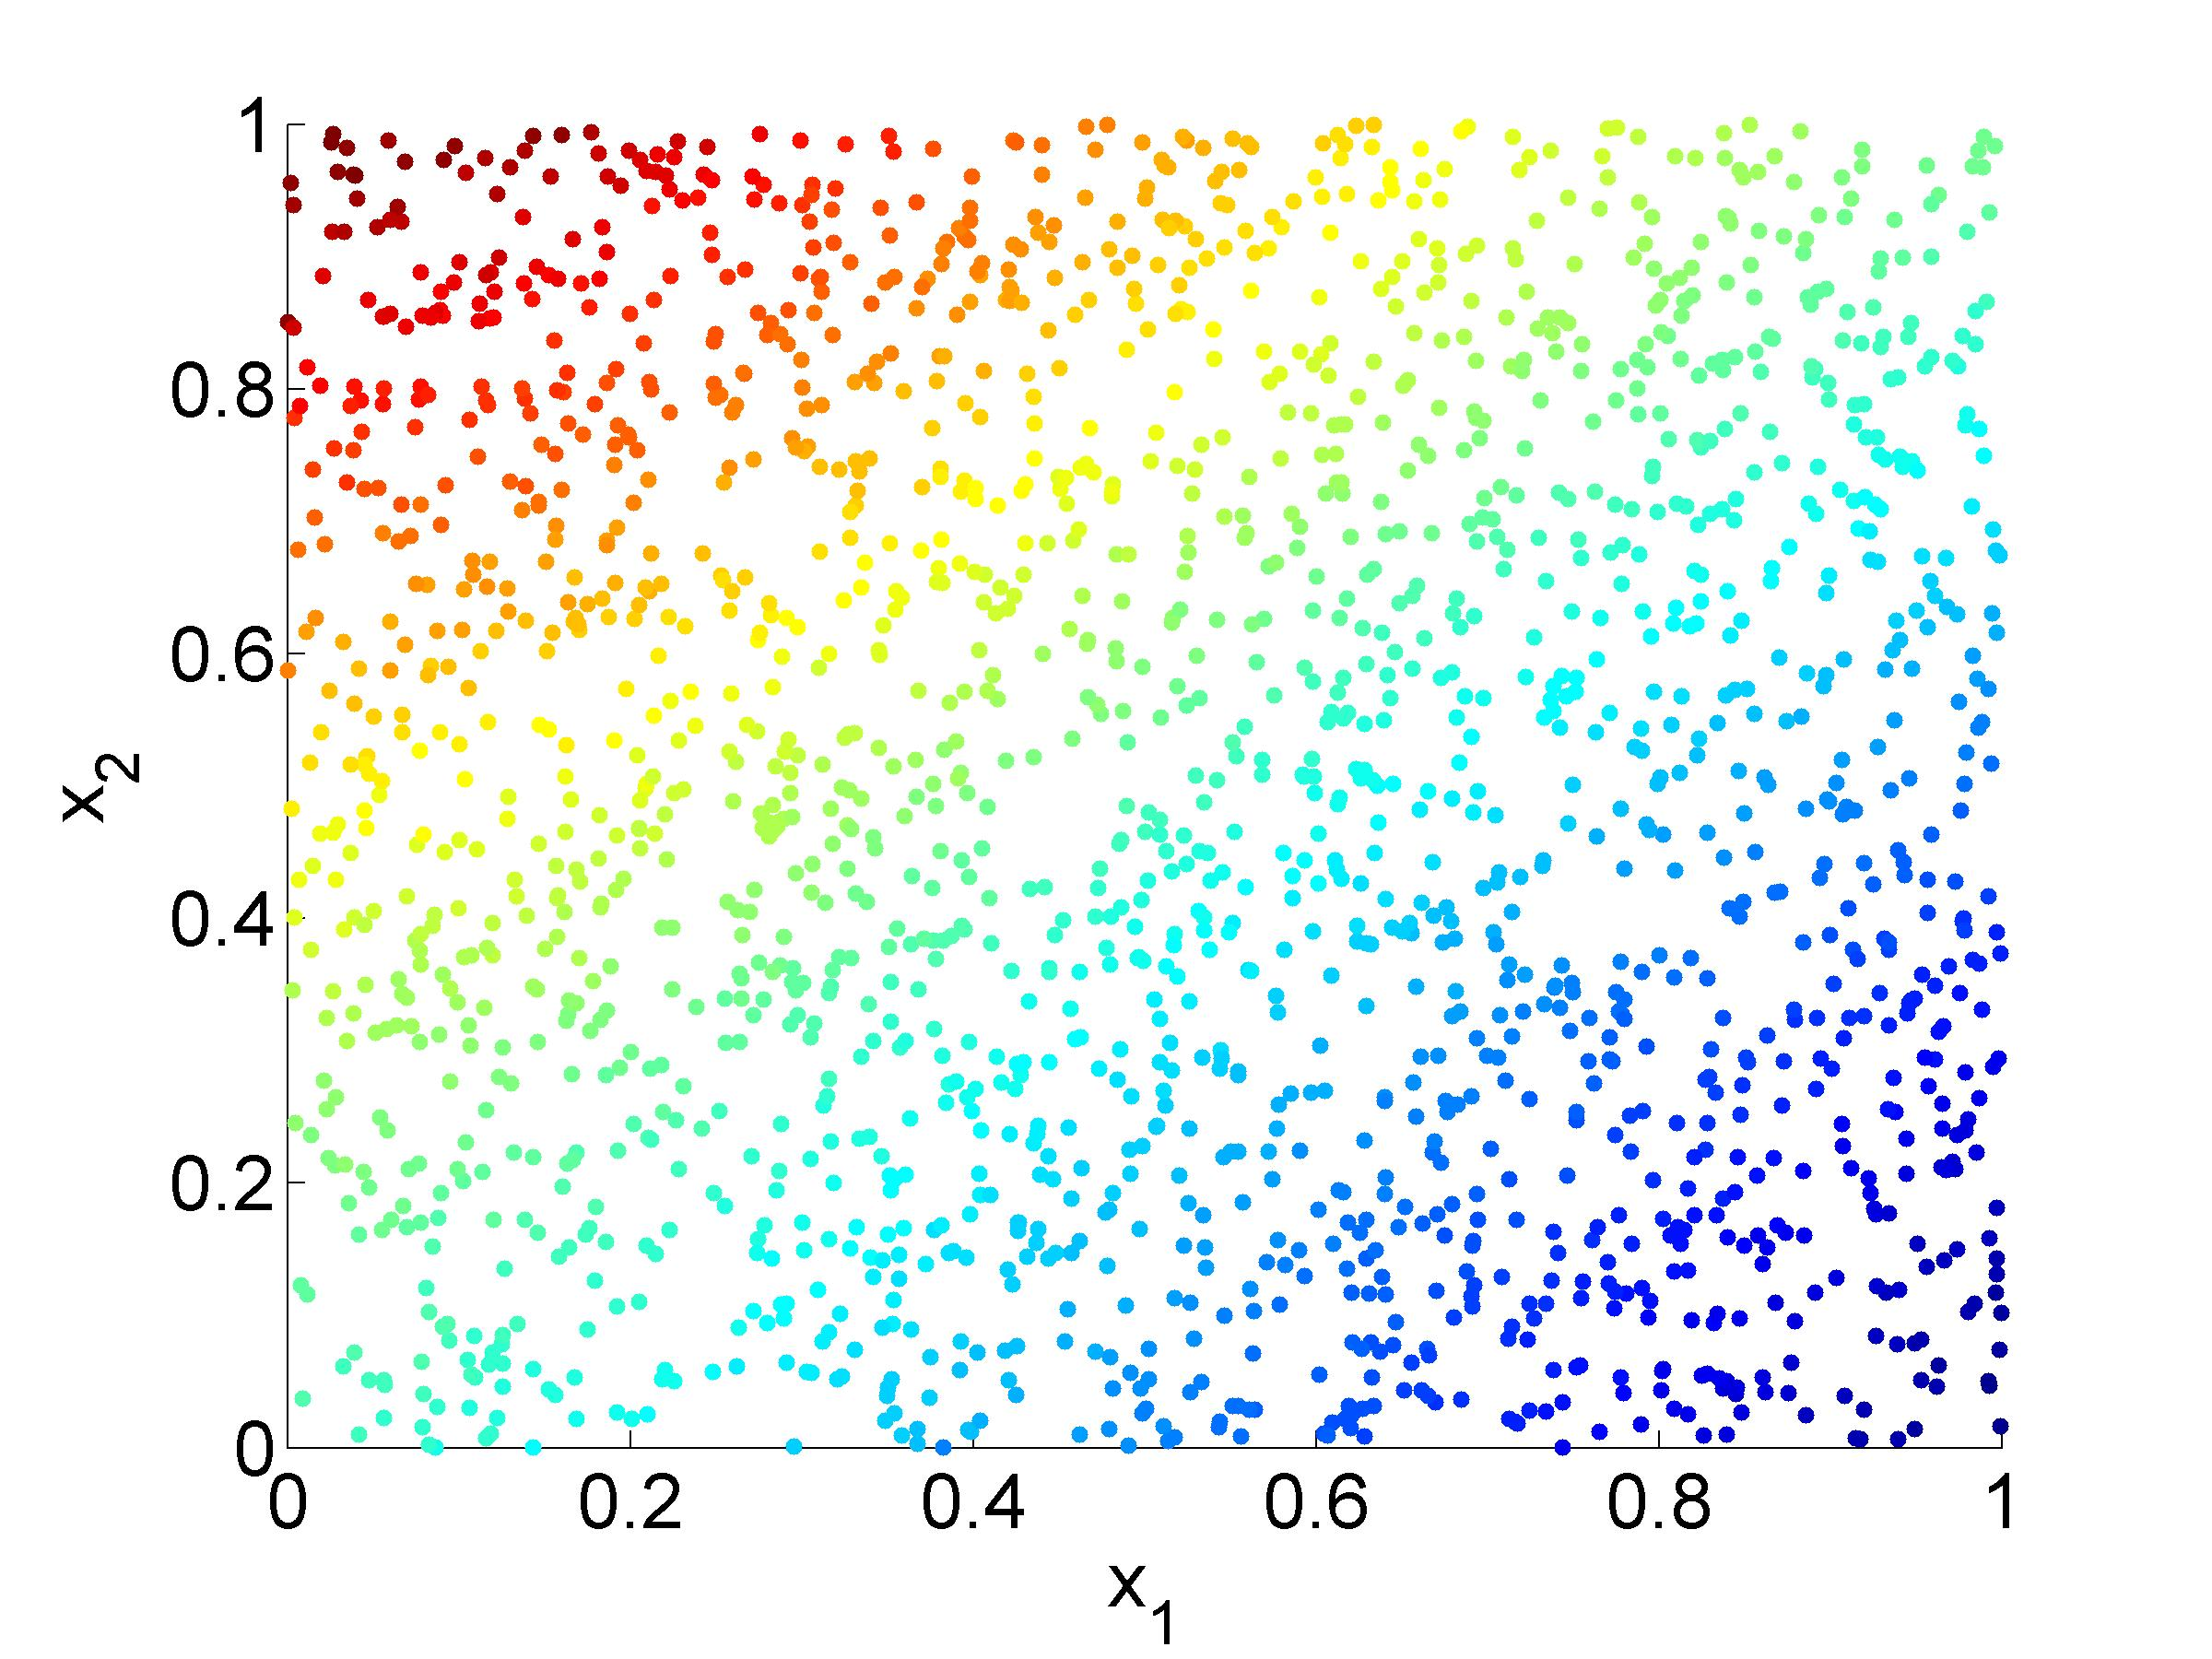
\includegraphics[width=0.3\textwidth]{xdata_noise1_colored_NIV1}
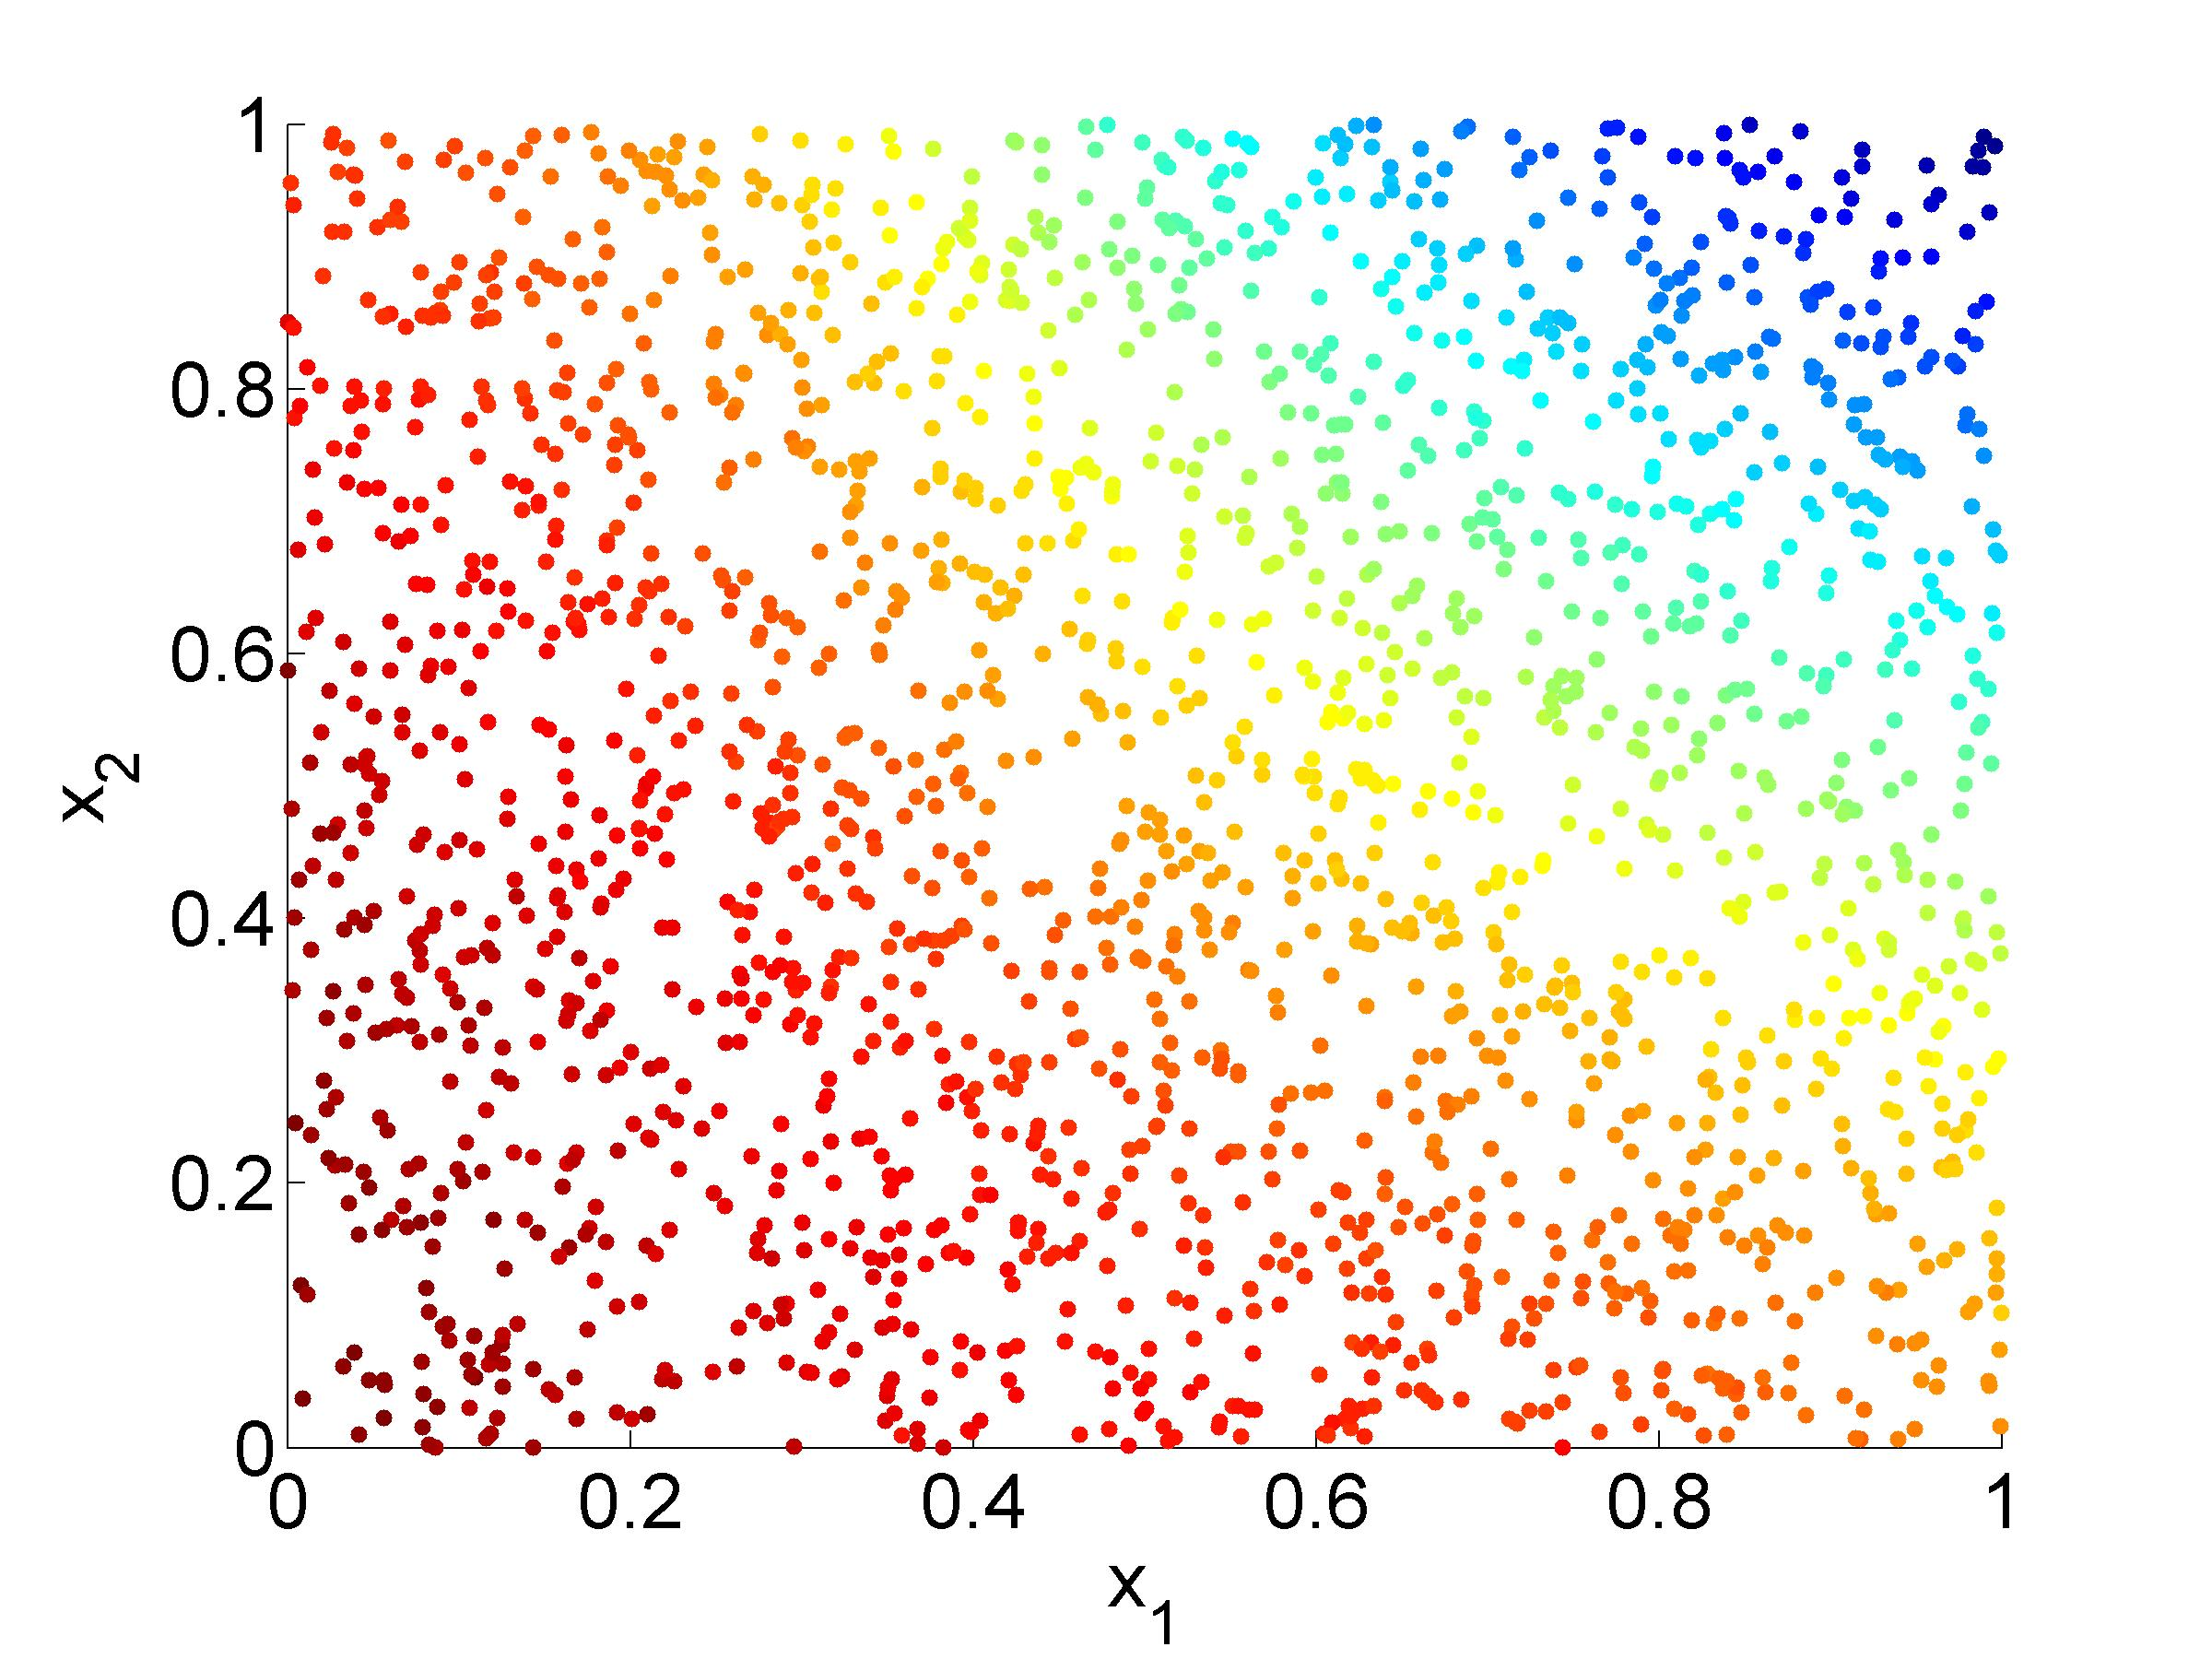
\includegraphics[width=0.3\textwidth]{xdata_noise1_colored_NIV2}
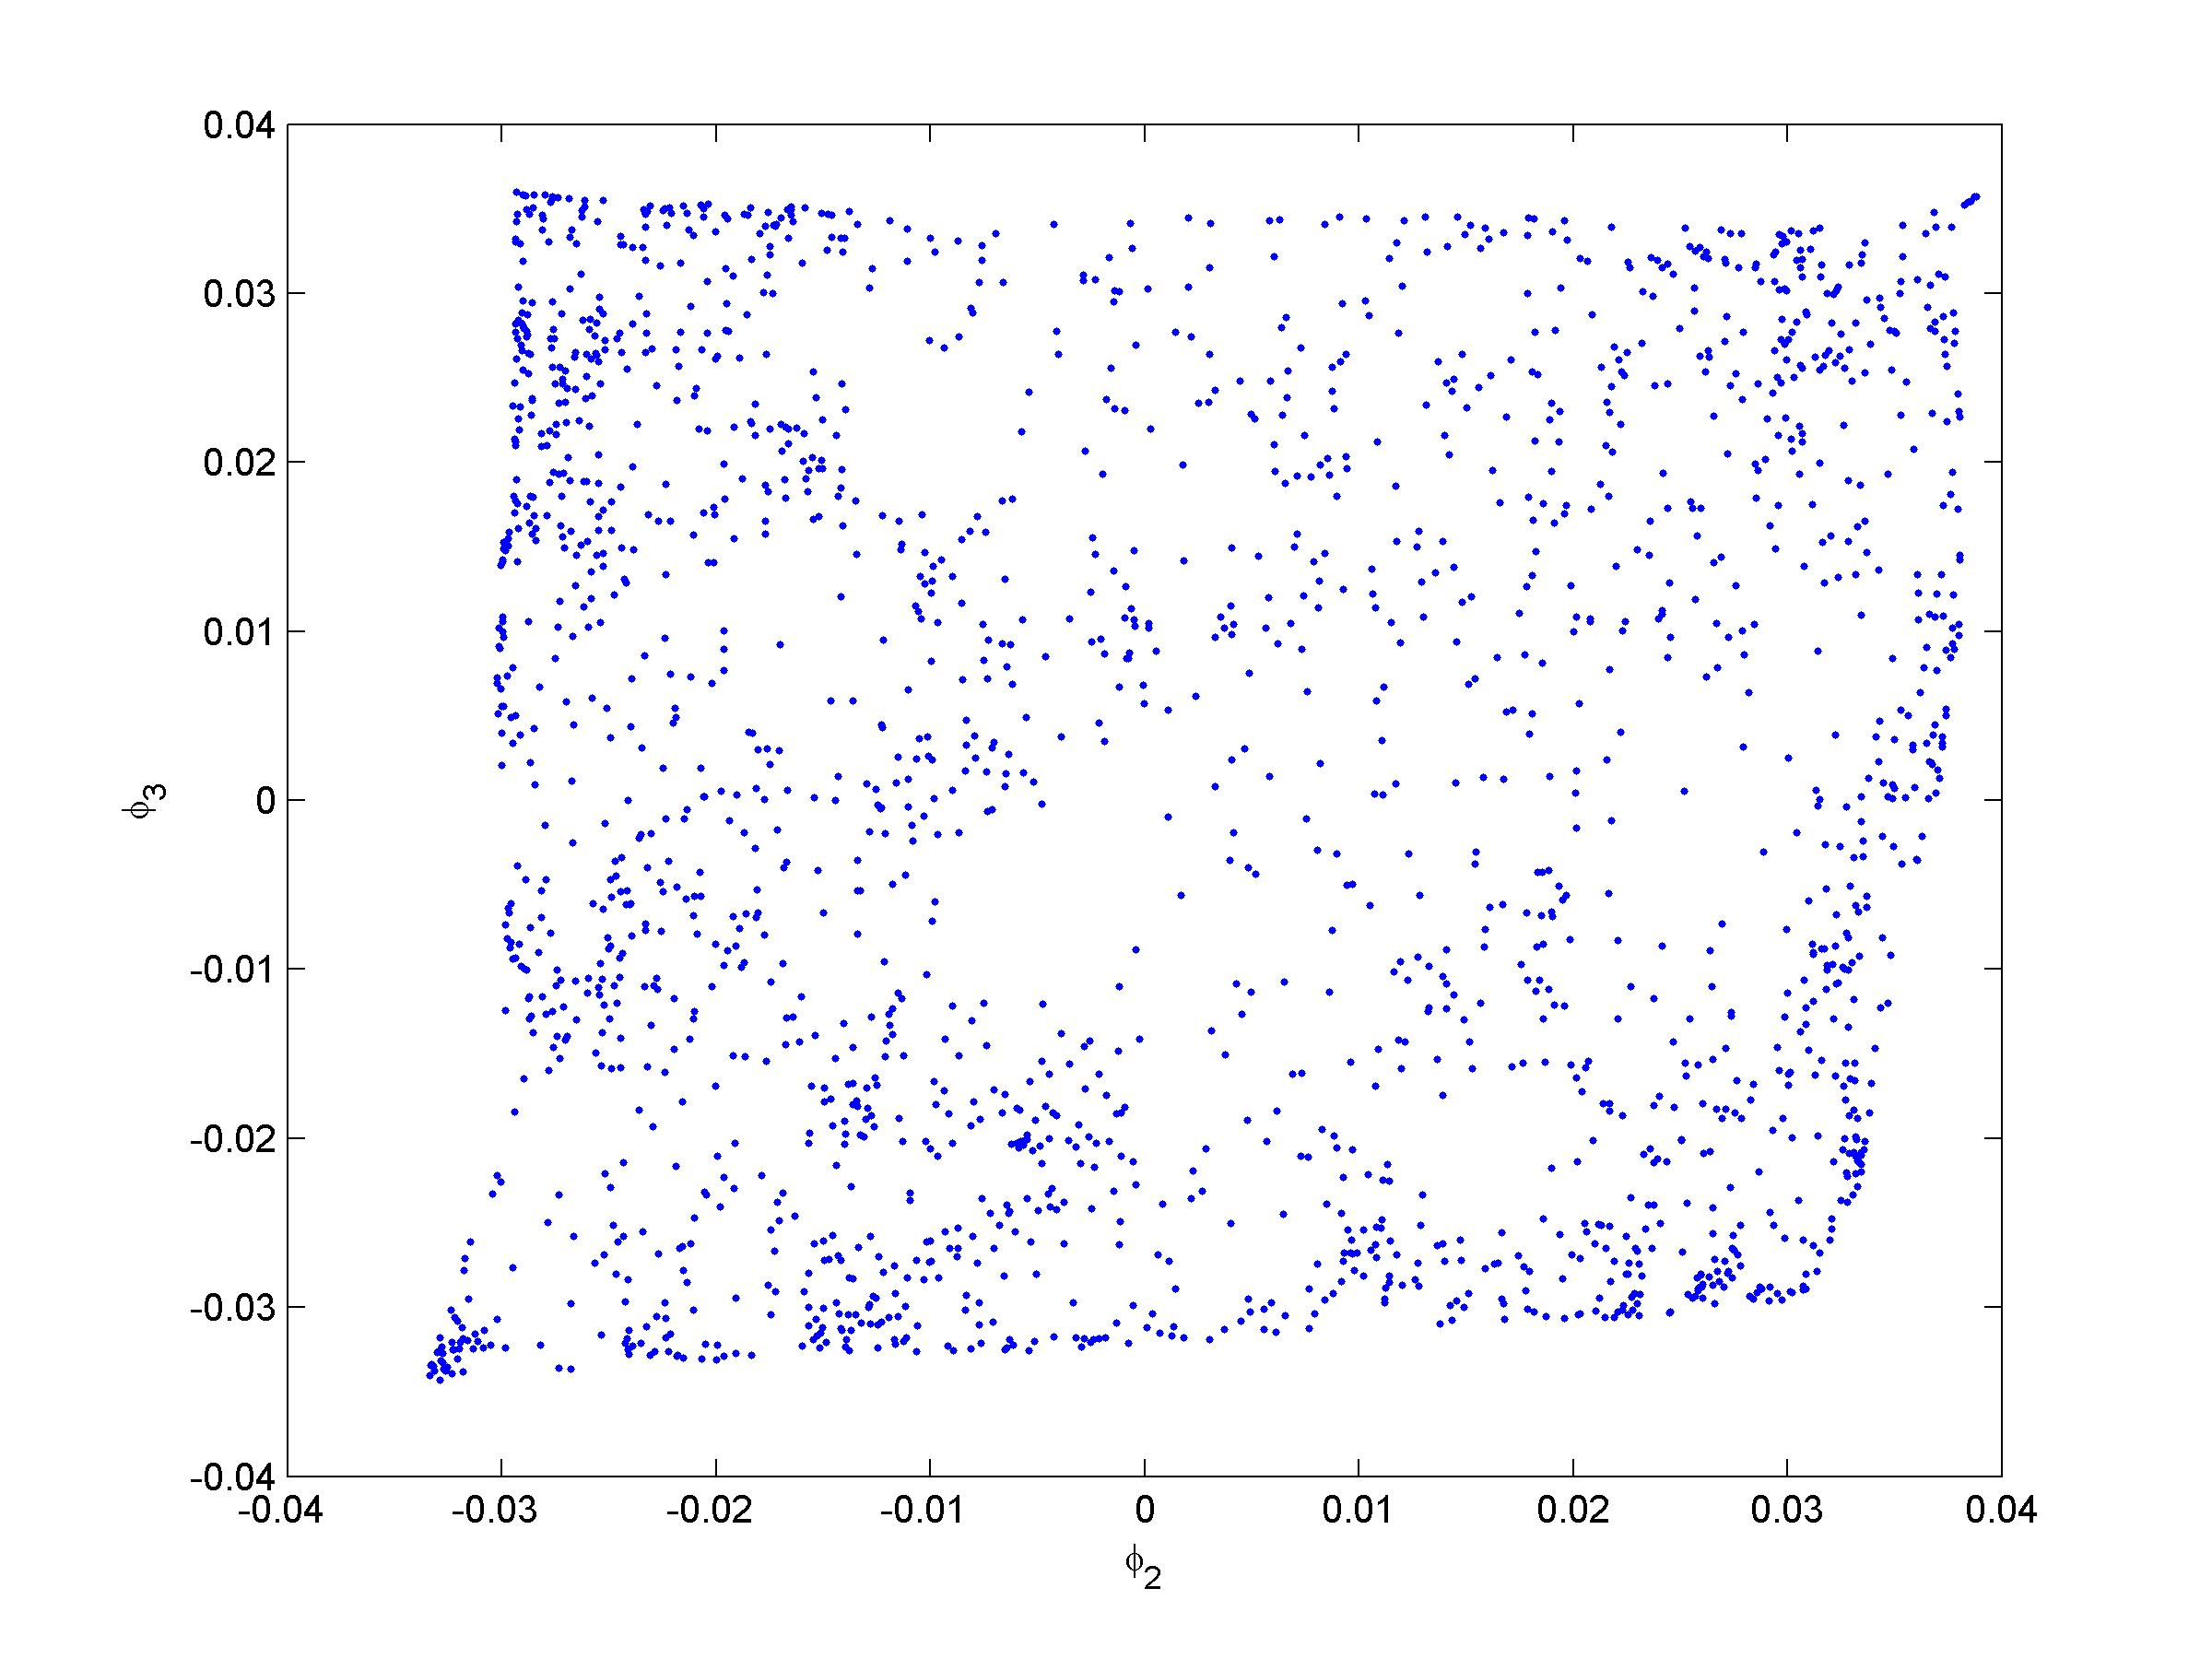
\includegraphics[width=0.3\textwidth]{embedding_noise1}
\caption{Data in ``true'' space ($x_1, x_2$), colored by the first (left) and second (center) nontrivial NIV. The NIV embedding is computed from the data in the ambient space with added noise ($z_1, z_2$, with $\sigma = 0.01$). Note that the parameterizations we obtain are the eigenfunctions that we expect for points sampled from the unit square. (right) Data plotted in first two (nontrivial) NIV. We (effectively) recover the unit square, i.e., the domain of the intrinsic variables. }
\label{fig:xdata_NIV_noise1}
\end{figure}

If $\sigma = 100$ (so the added noise is much larger than the noise in the original clouds), we obtain a parameterization shown in Figure \ref{fig:xdata_NIV_noise2} using NIV.
%
Now, the ellipses are a combination of the intrinsic varibale noise, and the ambient space noise, but the ambient space noise is {\em much} larger. 
%
Therefore, NIV only collapses the ambient space noise (not the intrinsic variable noise), and so we get something like the DMAPS coordinates, rather than the NIV. 

\begin{figure}[htb]
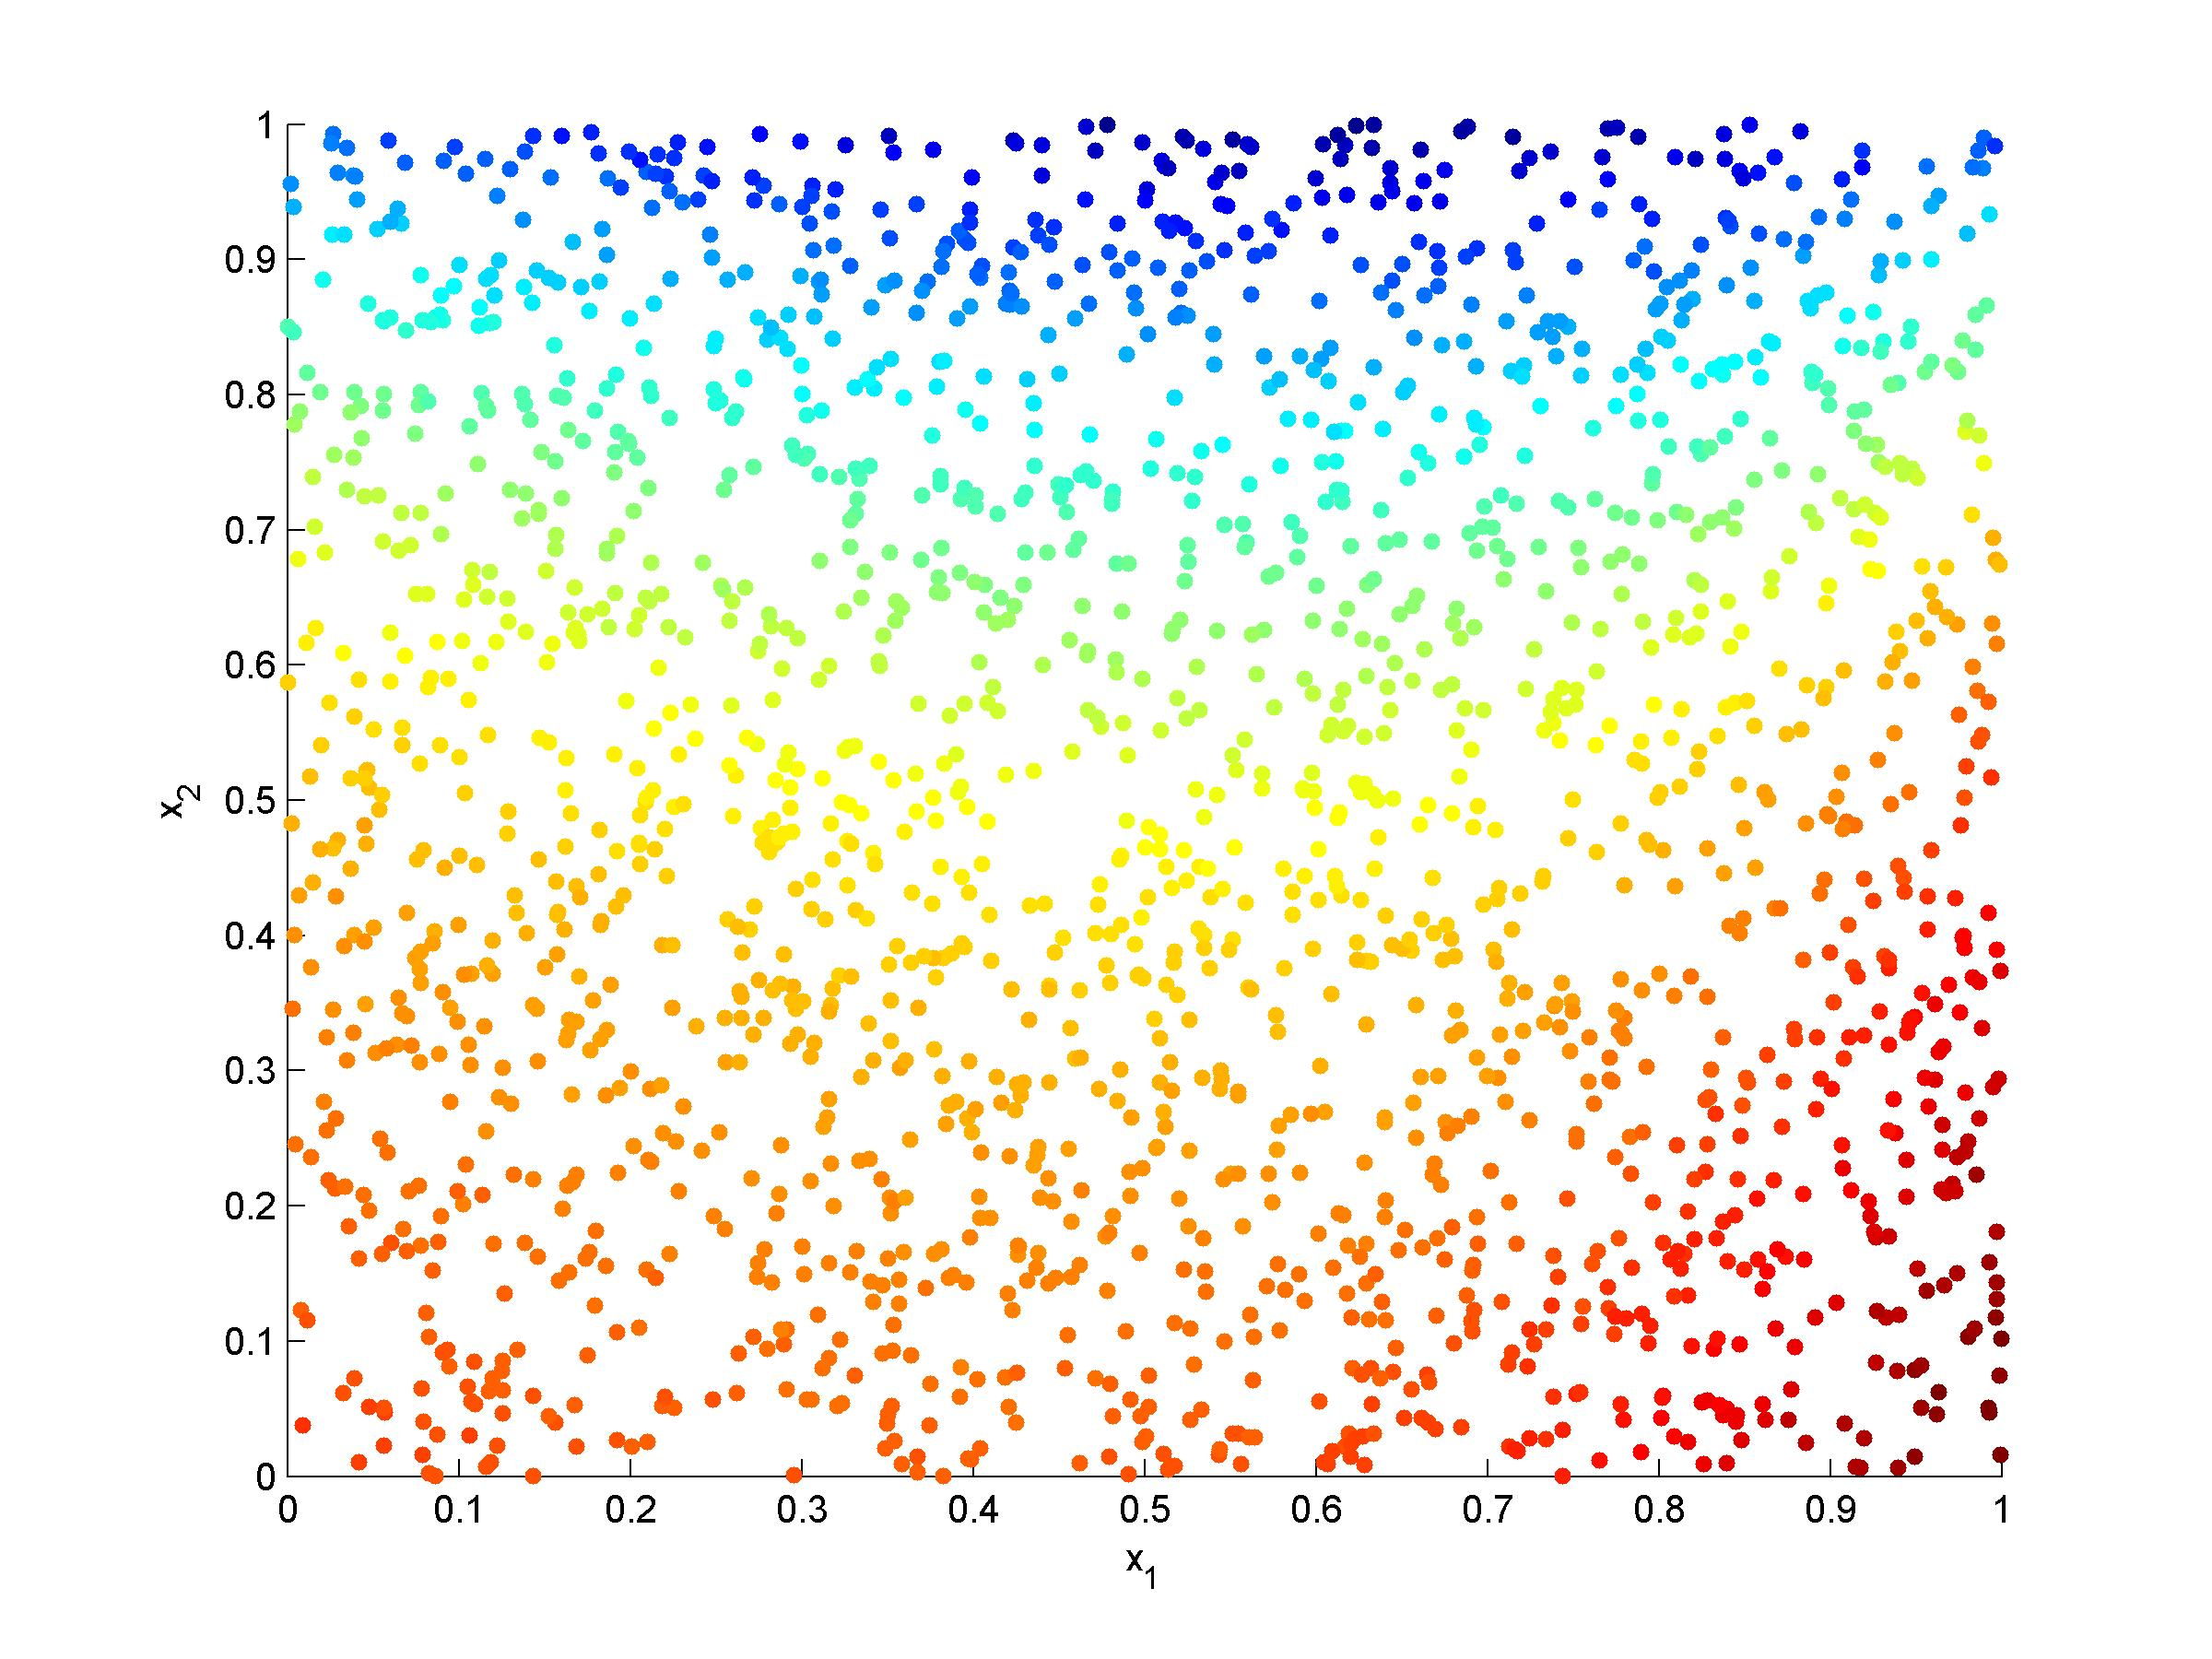
\includegraphics[width=0.3\textwidth]{xdata_noise2_colored_NIV1}
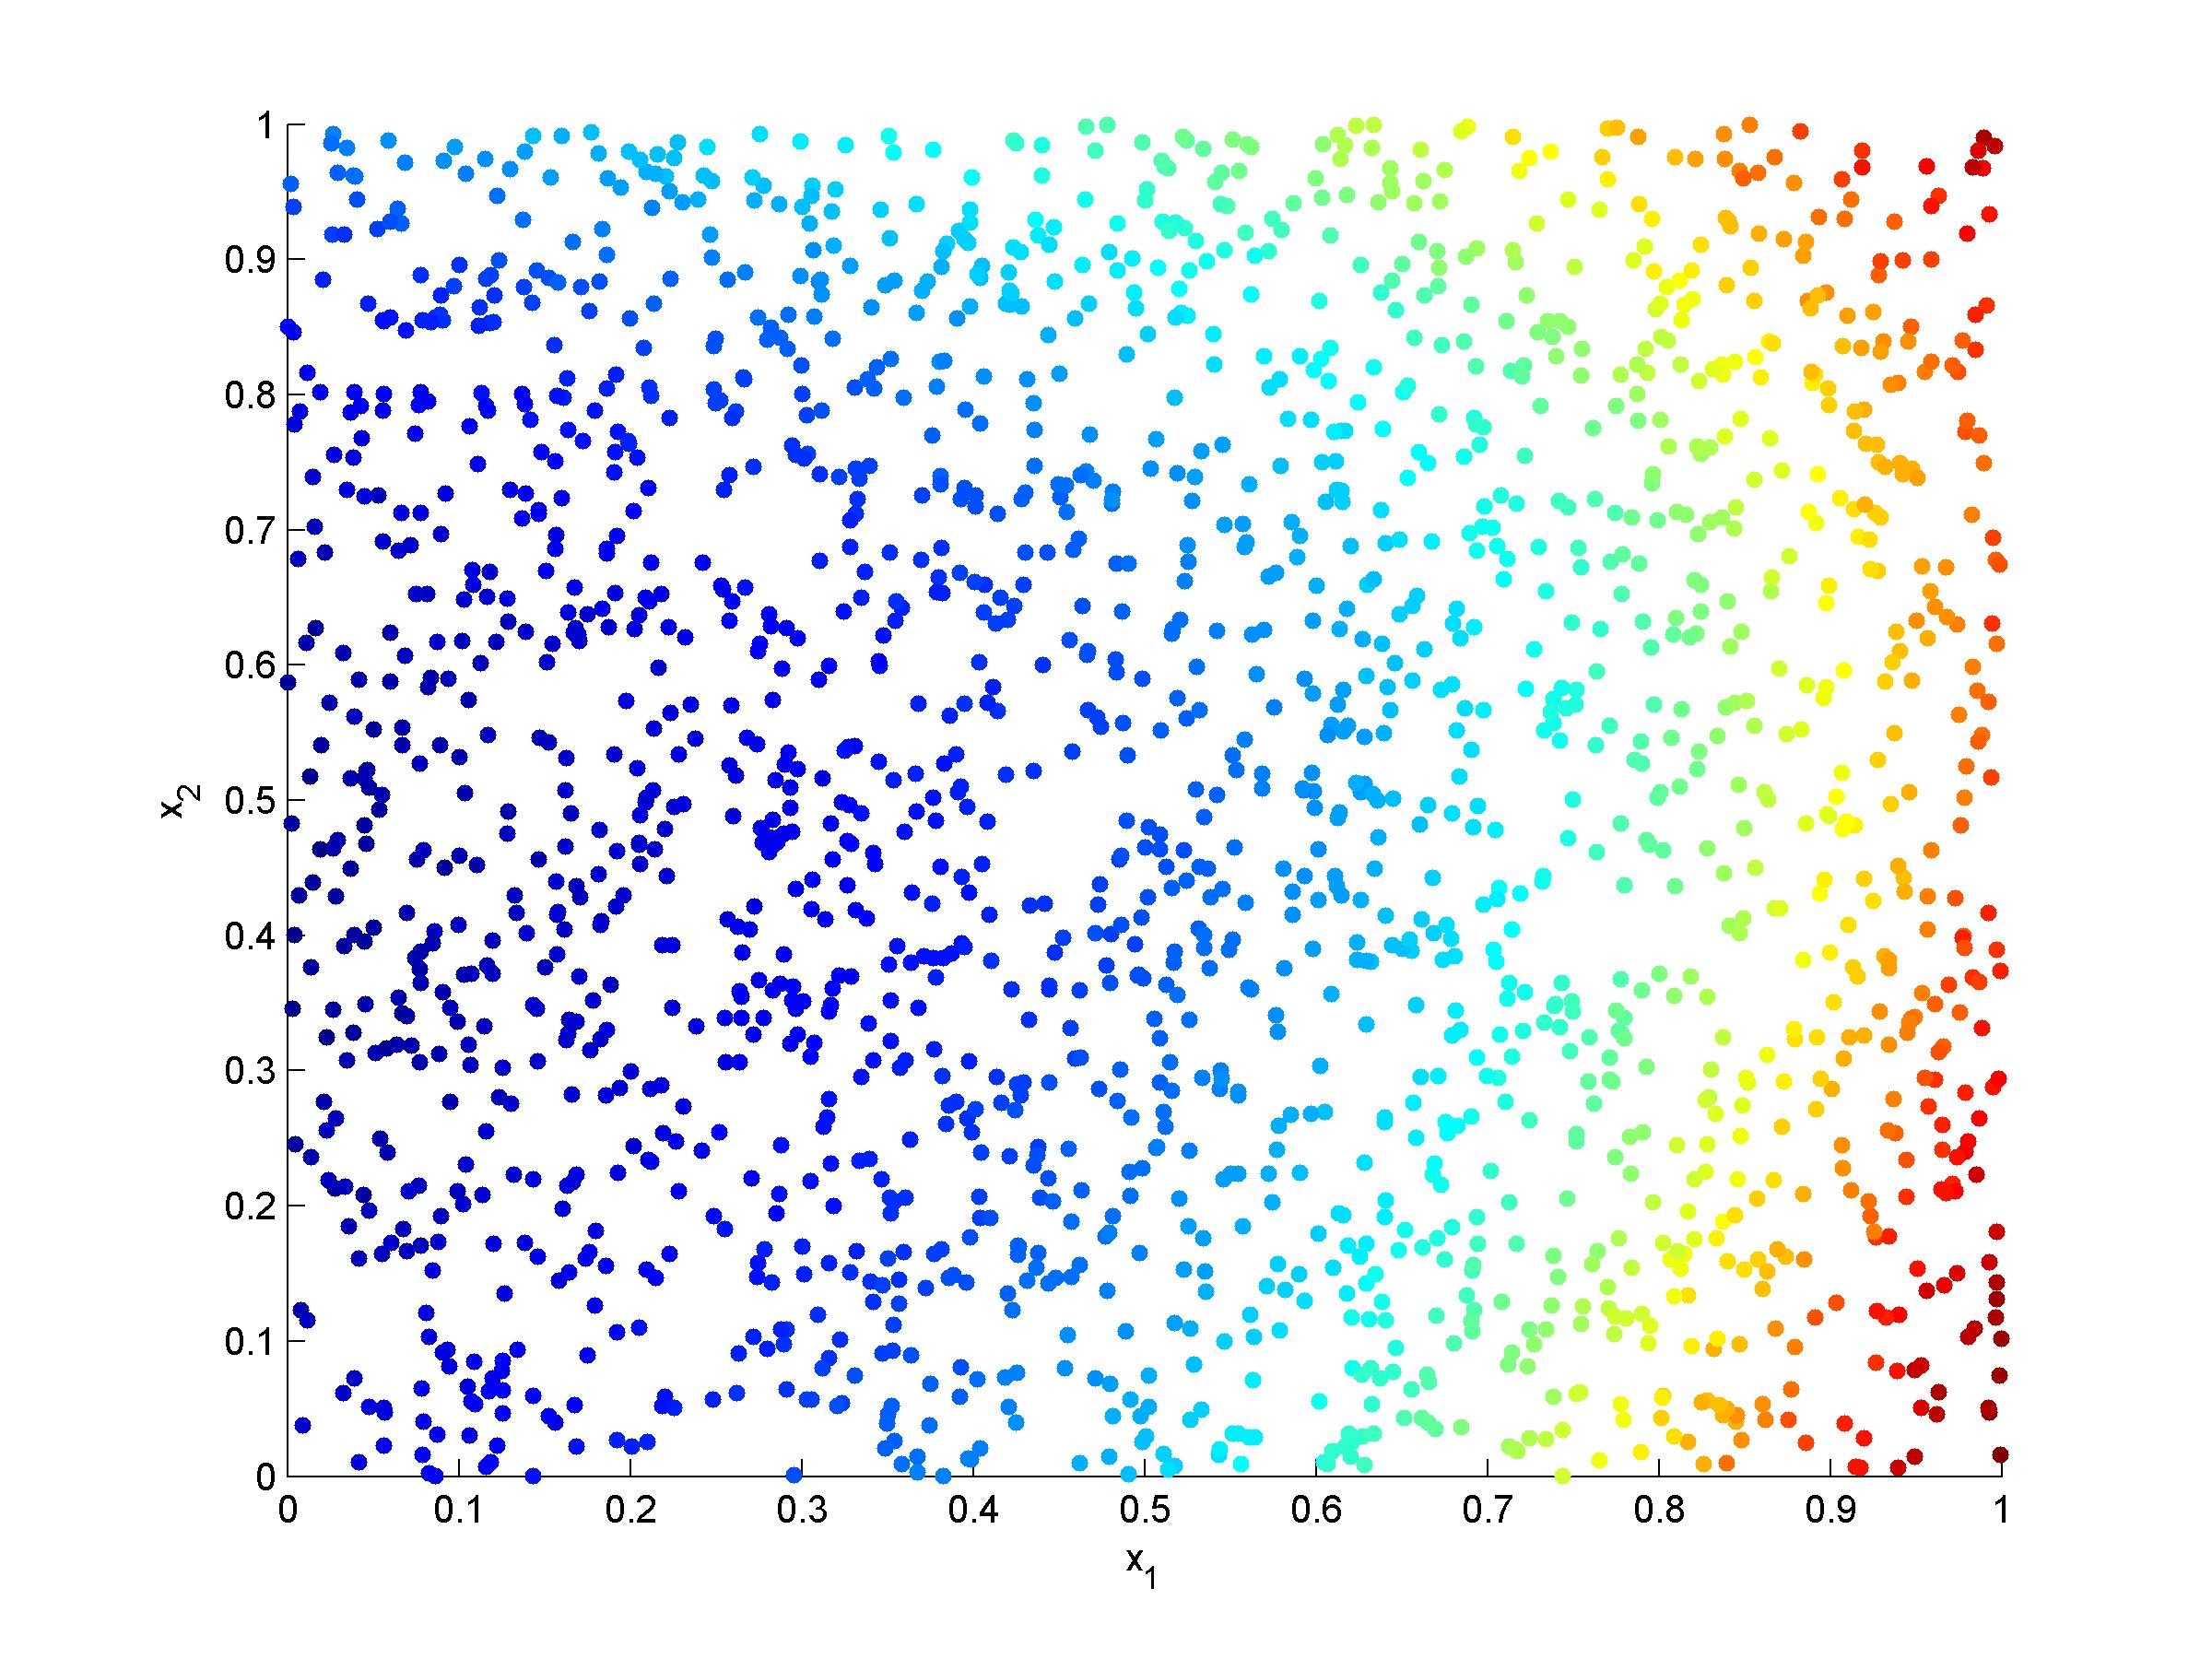
\includegraphics[width=0.3\textwidth]{xdata_noise2_colored_NIV2}
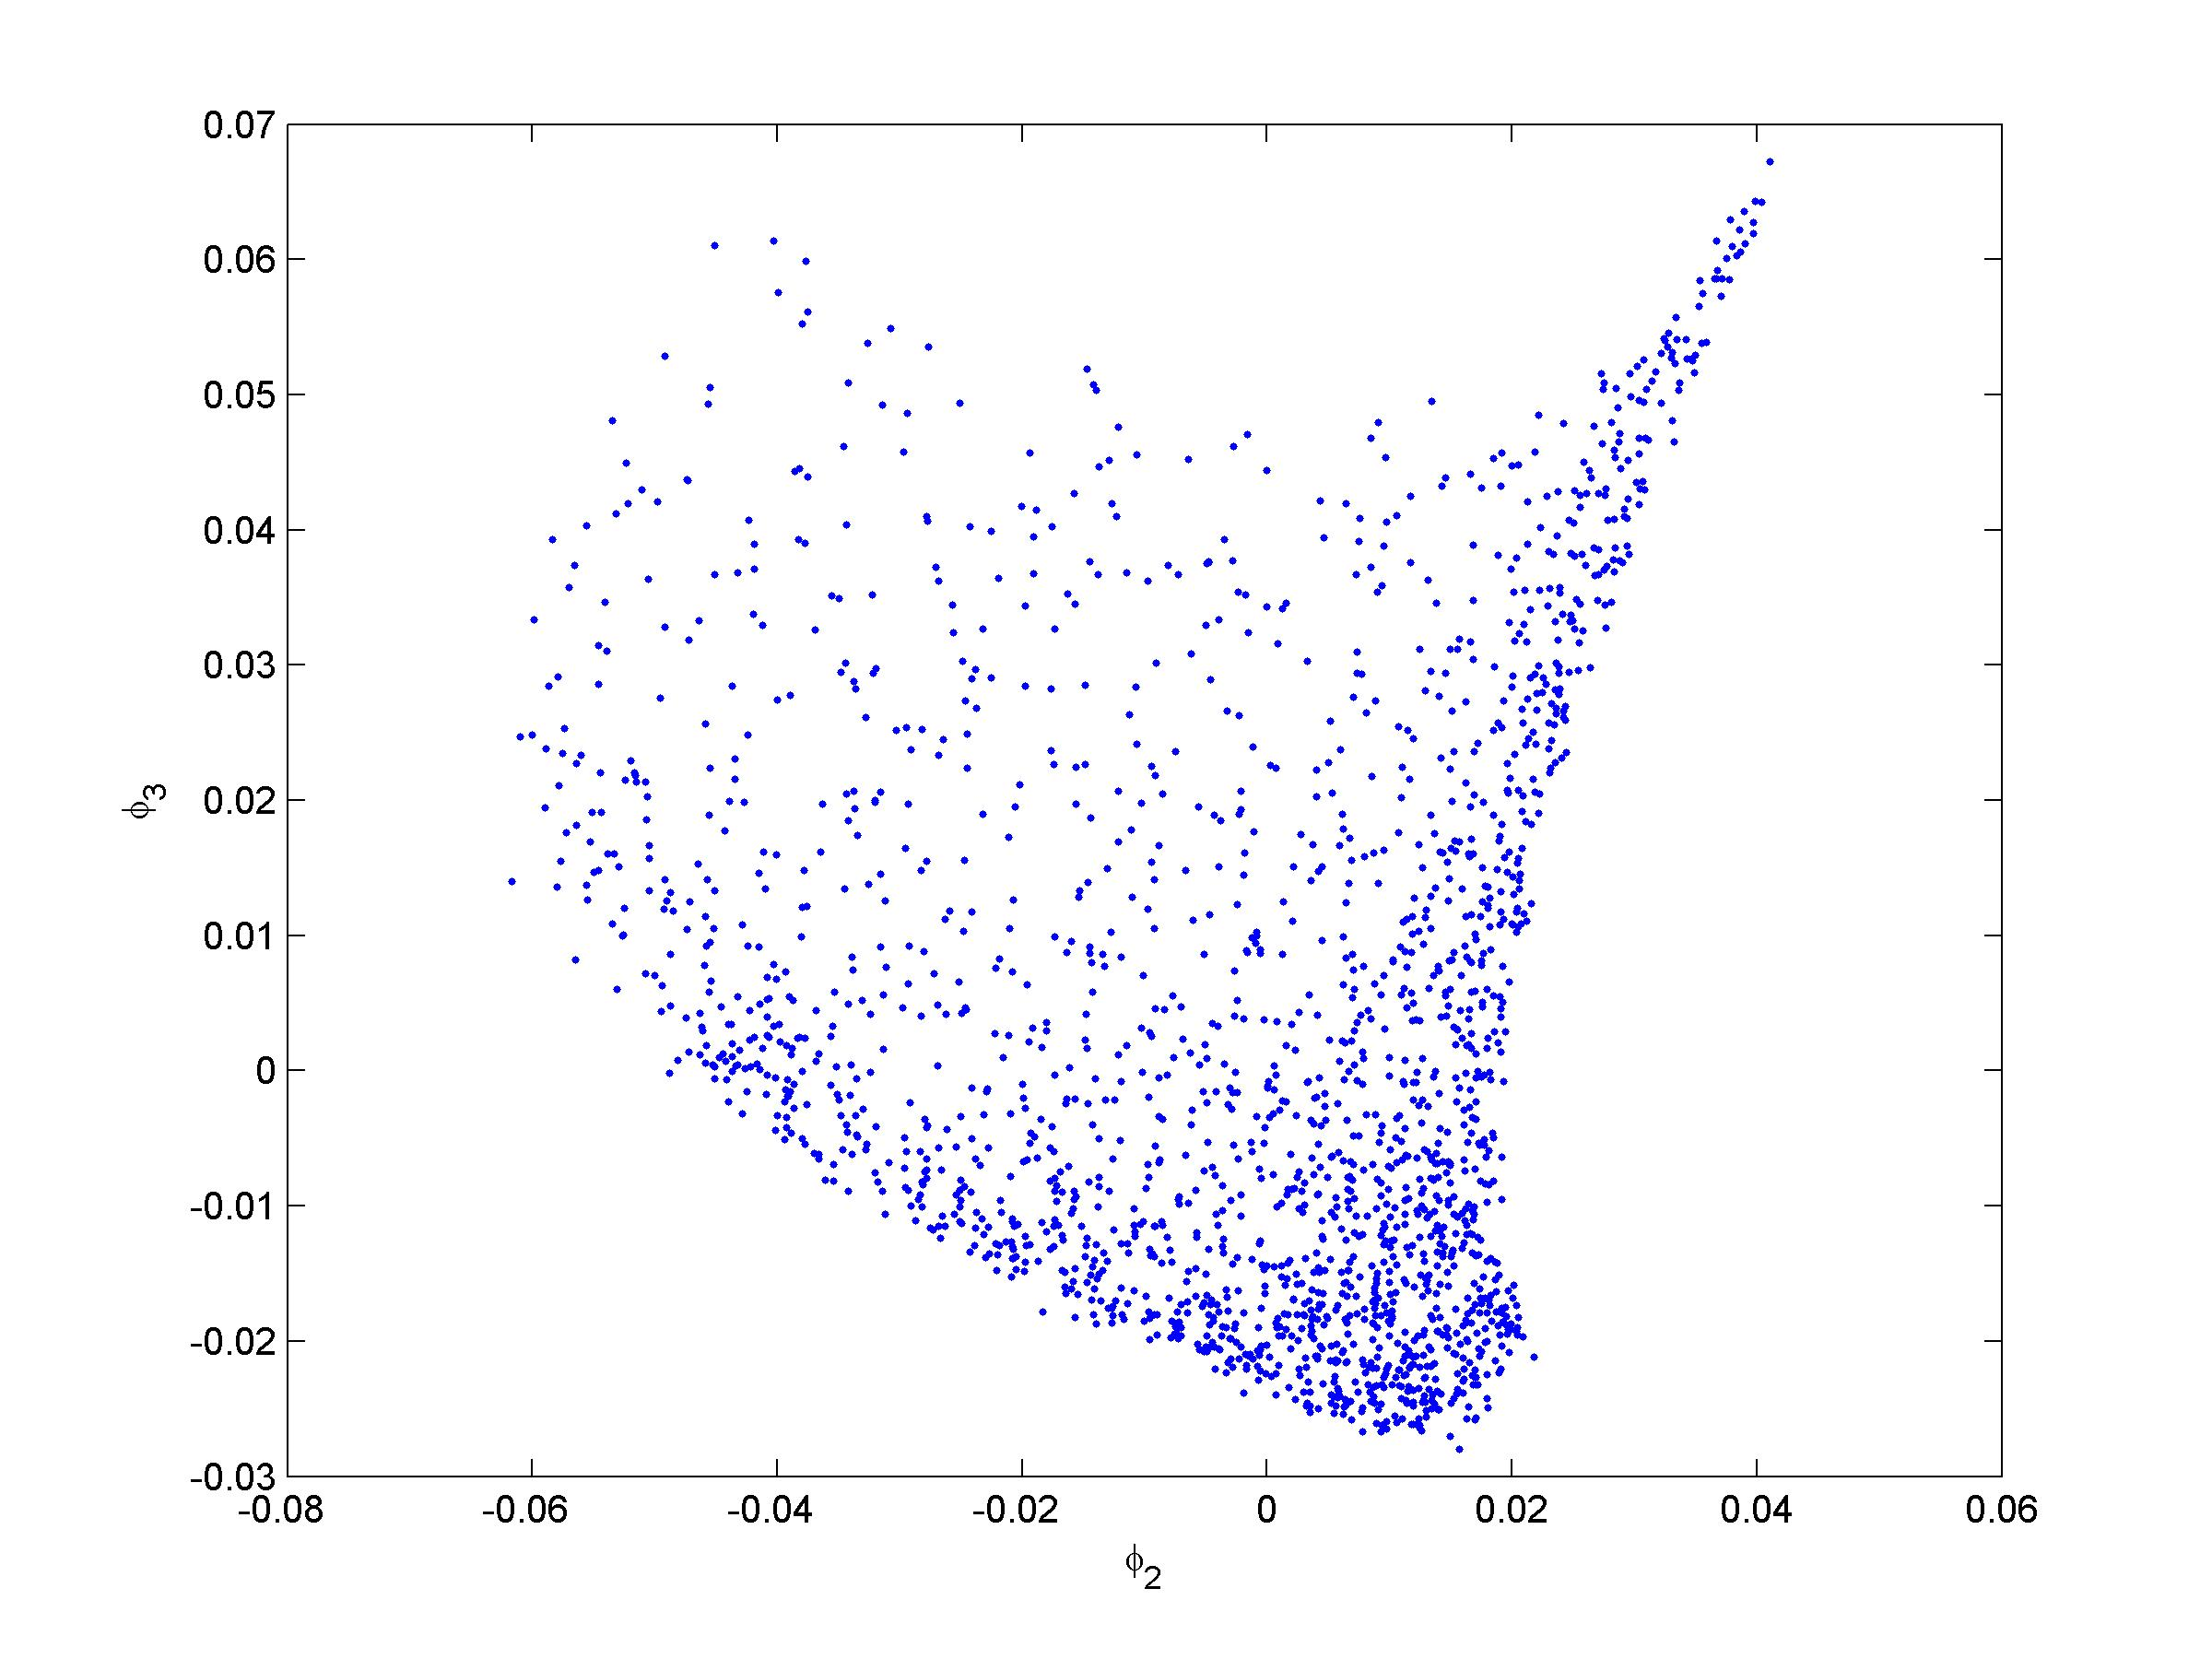
\includegraphics[width=0.3\textwidth]{embedding_noise2}
\caption{Data in ``true'' space ($x_1, x_2$), colored by the first (left) and second (center) nontrivial NIV. The NIV embedding is computed from the data in the ambient space with added noise ($z_1, z_2$, with $\sigma = 100$). Note that the parameterizations we obtain are not the eigenfunctions that we expect for points sampled from the unit square, but are now similar to the parameterizations obtained from DMAPS shown in Figure \ref{fig:xdata_dmaps}. (right) Data plotted in first two (nontrivial) NIV. We do {\em not} recover the unit square.}
\label{fig:xdata_NIV_noise2}
\end{figure}

\end{document}